\documentclass[11pt]{article}
\usepackage[sc]{mathpazo} %Like Palatino with extensive math support
\usepackage{fullpage}
\usepackage[authoryear,sectionbib,sort]{natbib}
\linespread{1.7}
\usepackage[utf8]{inputenc}
\usepackage{lineno}
\usepackage{titlesec}
\titleformat{\section}[block]{\Large\bfseries\filcenter}{\thesection}{1em}{}
\titleformat{\subsection}[block]{\Large\itshape\filcenter}{\thesubsection}{1em}{}
\titleformat{\subsubsection}[block]{\large\itshape}{\thesubsubsection}{1em}{}
\titleformat{\paragraph}[runin]{\itshape}{\theparagraph}{1em}{}[. ]\renewcommand{\refname}{Literature Cited}

\usepackage{amsmath,amsfonts,amssymb}
\usepackage[english]{babel}
\usepackage[latin1]{inputenc}
\usepackage[T1]{fontenc}
\usepackage{color}
\usepackage{float}
\usepackage{verbatim}
\usepackage{graphicx}
\usepackage{bm}
\usepackage{mathtools}
\usepackage{stmaryrd}
\usepackage{anyfontsize}
\usepackage{color}
\usepackage{subcaption}
% \usepackage{subfigure}

%%%%%%%%%%%%%%%%%%%%%
% Line numbering
%%%%%%%%%%%%%%%%%%%%%
%
% Please use line numbering with your initial submission and
% subsequent revisions. After acceptance, please turn line numbering
% off by adding percent signs to the lines %\usepackage{lineno} and
% to %\linenumbers{} and %\modulolinenumbers[3] below.
%
% To avoid line numbering being thrown off around math environments,
% the math environments have to be wrapped using
% \begin{linenomath*} and \end{linenomath*}
%
% (Thanks to Vlastimil Krivan for pointing this out to us!)

\title{On the dynamics of starvation, mortality, and the ephemeral nature of mammalian megafauna}

% This version of the LaTeX template was last updated on
% November 8, 2019.

%%%%%%%%%%%%%%%%%%%%%
% Authorship
%%%%%%%%%%%%%%%%%%%%%
% Please remove authorship information while your paper is under review,
% unless you wish to waive your anonymity under double-blind review. You
% will need to add this information back in to your final files after
% acceptance.

\author{Taran Rallings$^{1,\ast}$ \\ 
Christopher P. Kempes$^{2}$ \\ 
Justin D. Yeakel$^{1}$}

\date{}

\begin{document}

\maketitle

\noindent{} 1. School of Natural Sciences, University of California Merced, Merced, California 95343, USA;

\noindent{} 2. Santa Fe Institute, Santa Fe, New Mexico 87501, USA;

% \noindent{} 3. Middle Eastern Technical University, Çankaya, Ankara 06800, Turkey.

\noindent{} $\ast$ Corresponding author; e-mail: trallings@ucmerced.edu.

% \noindent{} $\dag$ Deceased.

\bigskip

\textit{Manuscript elements}: Figure~1, figure~2, table~1, online appendices~A and B (including figure~A1 and figure~A2). Figure~2 is to print in color.

\bigskip

\textit{Keywords}: Examples, model, template, guidelines.

\bigskip

\textit{Manuscript type}: Article. %Or e-article, note, e-note, natural history miscellany, e-natural history miscellany, comment, reply, invited symposium, or historical perspective.

\bigskip

\noindent{\footnotesize Prepared using the suggested \LaTeX{} template for \textit{Am.\ Nat.}}

%\linenumbers{}
%\modulolinenumbers[3]

\newpage{}

\section*{Abstract}

Great Abstract

\newpage{}


\section*{Introduction}

% [P1: consumer-resource systems and allometry... energy compartments...paleo]
Consumer-resource interactions form the network of energy flow within ecosystems. The rates at which energy flows and pools are determined in large part by the body-mass of the consumers involved in the interactions. These allometric relationships between consumer body-mass and energy use constrain energy intake, storage, and metabolism as well as the population dynamics that rely on them. The scaling of the ratio of fat to non-fat mass in mammals, for example, is central to understanding how these physiological constraints influence population level dynamics. This ratio of fat to non-fat mass is the relative weight of energy storage to metabolism in an individual. The ratio scales predictably and positively with body-mass which creates size-structured patterns like starvation tolerance. The constraints imposed by these physiological allometries on population dynamics allow us to make predictions about populations that we cannot directly observe. This is notably important for understanding paleo-ecosystems as our knowledge is often limited to body-mass and taxa. By combining energetic models with allometric parameters we can approximate the energy needs and use of extinct consumers and interrogate sized-structured ecological patterns such as the megafaunal extinction at the terminal Pleistocene. 


% [P2: different sources of mortality]

Population outcomes, downstream of the energetic constraints imposed by allometry, emerge from the balance of reproduction and mortality experienced by the population. Reproduction has a single source whose rate, in mammals, decreases with body-mass. The mortality that reproduction must balance has a variety of forms which do not all scale in the same manner. In order to make predictions about population outcomes through this energetic lens we must understand the form and scaling of these diverse mortalities: starvation, survivorship, predation, and harvest.  Starvation through resource limitation is a product of the ratio of fat to non-fat mass and environmental conditions. As the ratio increases with body-mass, the rate of starvation mortality decreases with body-mass. Survivorship mortality arises from the array of risks faced by a consumer both in its initial year of life and as it ages.  The rate of survivorship mortality decreases with consumer mass. Predation mortality is faced by consumers being preyed upon by predators. The rates of predation mortality decrease with body-mass as the range of predators capable of hunting the consumer decreases. Harvest mortality arises principally from human activity. It can take the form of hunting but is size-structured mortality that does not face the same rate and allometric constraints as the consumer-resource interactions found in nature. A human culture specialized in hunting large mammals imposes a size-structured mortality on consumer populations that does not obey the scaling seen in other mammalian consumer-resource interactions. Reproduction and these diverse mortalities interact to create population level outcomes and, through their body-mass scalings, impose constraints on the body size of consumers.

% [P3: constraints of size]

The patterns of body-size and abundance seen in nature are a product of energetic allometry, reproduction, and multiple sources of mortality. Most of the energetic allometries experienced by terrestrial mammals have rates decreasing with body-mass. As a result, smaller mammals have higher reproductive rates as well as higher rates of mortality through starvation, survivorship, and predation. Larger mammals have lower reproductive rates but experience lower rates mortality through starvation, survivorship, and predation. Both large and small mammals can then persist in nature under the conditions where their respective rates of mortality and reproduction are balanced despite being of different magnitudes. The significance of the difference in magnitude, large consumers having lower reproductive rates, is that larger mammals are then much more vulnerable to sources of mortality that do not obey this negative scaling pattern. A size agnostic mortality, applied across a community, will have a more negative impact on large mammals.  A size-structured extinction event, like the loss of megafauna seen at the end of the Pleistocene, must result from a force of mortality that scales with body-mass in a manner unlike the existing sources. 

% [P4: Here we]

Here we...

% What is the background for this paper? 
% What are the questions?

% (Taran’s stream of consciousness introduction)

% The goal of this paper is to understand how multiple sources of mortality interact in determining densities for consumer species and to build a (mostly) mechanistic consumer-resource model that can be extended to look at paleo food webs. The NSM provided a mechanistic framework for thinking about herbivorous mammals and their resources, tying all the consumer parameters to well documented allometric relationships. The limitation of that model is that it tracks two consumer states: full and starved. A second consumer state creates difficulties for parameterizing mortalities over the two states and leads to computational limitations at the complex food-web level. 

% The NSM is a particularly useful foundation for paleo food-webs because the mechanistic parameterization is entirely allometric. When building models for paleo-ecosystems a persistent limitation is how to accurately decide on parameter values for interactions you cannot observe or ecosystems that no longer exist or species that are completely extinct. We cannot collect this data from the field so we need to build on known relationships between body-mass and energy for accurate parameterization. \\




% \emph{Introduce the NSM}

% The two dimensional consumer-resource model used here is a modification of the three dimensional “nutritional-state model”(NSM) (Yeakel et al 2018). In the NSM the consumer, assumed to be a herbivorous mammal, has two states: a full state and a starved state. The full state is capable of reproduction and experiences no mortality. The starved state is not capable of reproduction and faces mortality. The transition rates between the full and starved states are a function of of resource density. More specifically, the transition rates are a function of the proportional fullness of resource carrying capacity. When the resource is at carrying capacity, transitions between the full and starved states become unidirectional, moving from starved to full. When the resource is extinct, the transition term from starved to full drops out, all consumers transition to the starved state, and then die. \\

% \emph{Explain the two-dimensional model}

% This NSM has been modified by collapsing the full and starved consumer states into a single consumer population. This modification causes the transition rates between the full and starved states to drop out and leave only intrinsic rates of reproduction and mortality. To capture the implicit effects of starvation these reproduction and mortality rates are modified by the resource density as a proportion of it’s carrying capacity. This is structurally similar to the role resource density plays in the NSM serving to modify transition rates between the full and starved states. Here a resource at its carrying capacity means that the consumer can reproduce at it’s maximum rate. As the proportional resource density decreases the effective consumer reproductive rate decreases in the same way. The starvation mortality rate of the consumer is a function of proportional resource density $(1-R/k)$ as well . When the resource is at carrying capacity the starvation mortality term drops out and no mortality by starvation occurs. As proportional resource density is reduced the starvation mortality rate increases. Eventually, at resource extinction $R=0$, the starvation mortality rate reaches its maximum. \\


% \emph{Explain how rates are mechanistic}

% The vital rates in our model have time scales based on the general ontogenetic growth model in (West et al 2001). The rates vary as a function of the energetics of building and maintaining somatic tissue in both adults and juveniles. Building the model in this way allows us to mechanistically consider the affects of metabolism and by extension of organismal body-size.

% *** Explain in more detail in methods. ***









\section*{Results and Discussion}
\subsection*{Allometric Consumer-Resource Model}
%Description of the model
% \noindent {\bf Allometric Consumer-Resource Model} 
We model a consumer-resource interaction, where the resource density $R$ (g/m${}^2$) grows logistically with intrinsic growth rate $\alpha$ to a carrying capacity $k$, and declines due to consumption by an herbivore consumer population density $C$ (g/m${}^2$) (Eq. \ref{eq:2d}).
Consumed resources govern both consumer somatic maintenance and reproduction. 
The rate of consumption to fuel somatic maintenance is given by $\rho$, and is independent of resource density, as these are invariant requirements of the consumer population \citep{yeakel2018dynamics}.
In contrast, the rate of consumption to fuel reproduction is proportional to resource density and is given by $\lambda_C(R)/Y_C$, where $\lambda_{\rm C}(R)$ is the consumer growth rate and $Y_{\rm C}$ is the yield coefficient of the consumer describing the grams of consumer produced per gram of resource consumed (see Methods).
% We assume the consumer growth rate
% , and the consumer yield coefficient describes the grams of consumer produced per gram of resource consumed (see Methods).
The consumer's growth rate $\lambda_C(R)$ follows Michaelis-Menton (Type II) kinetics as a function of the resource density $R$, where the maximum growth is $\lambda^{\rm max}_{\rm C}$ and the resource half-saturation density is $\hat{k} = k/2$, such that 
\begin{equation}
    \lambda_{\rm C}(R) = \lambda^{\rm max}_{\rm C}\left(\frac{R}{\hat{k}+R}\right).
\end{equation}
% As the resource diminishes, consumer reproduction is slowed.

While the consumer population density grows at rate $\lambda_{\rm C}(R)$, we assume for now that consumer mortality is purely a function of starvation, where the rate of starvation $\sigma(1-R/k)$ increases as resources become scarce.
In this context, $\sigma$ can be interpreted as the maximal starvation rate that occurs when the environment is devoid of resources.
The full system describing resource and consumer dynamics is then given by
\begin{align}
    \frac{{\rm d}}{{\rm d}t}C &= \lambda_{\rm C}(R)C- \sigma \left(1 - \frac{R}{k} \right)C, \nonumber \\ 
    \frac{{\rm d}}{{\rm d}t}R &= \alpha R \left(1 - \frac{R}{k} \right) - \left(\frac{\lambda_{\rm C}(R)}{Y_{\rm C}} + \rho \right)C.
    \label{eq:2d}
\end{align}
The dynamic outcomes of this system of equations include two trivial steady states at $(R^*=0, C^*=0)$ and $(R^*=k,C^*=0)$, and one internal steady state where both the consumer and resource population coexist.
Because the internal steady state cannot be concisely written, we do not report it here (but see [repository] for code).
% \begin{align}
%     C^* &= \alpha k\frac{2\lambda^{\rm max}_{\rm C}\sigma Y_{\rm C}}{(2\lambda^{\rm max}_{\rm C}+\sigma)(2\lambda^{\rm max}_{\rm C} \sigma + (2\lambda^{\rm max}_{\rm C}+\sigma)Y_{\rm C}\rho)} \nonumber \\ 
%     R^* &= k \frac{\sigma}{2\lambda^{\rm max}_{\rm C} + \sigma},
%     \label{eq:2dss}
% \end{align}
% where both the consumer and resource population coexist.

The rate laws describing resource consumption as well as consumer growth and mortality all vary as a function of consumer body mass $M_{\rm C}$, where the consumer is assumed to be a mammalian herbivore, and the resource is an unspecified plant functional group with characteristic growth rate $\alpha$, carrying capacity $k$, and energy density $E_d$. %(see methods for derivations of allometric rate laws).
% While we describe the detailed derivations of allometric rate laws in methods (see methods), it is useful to briefly summarize how consumer rates scale with mass.
We approach the derivation of vital rates with respect to consumer mass by solving for multiple timescales associated with ontogenetic growth, maintenance, and expenditure.
The growth of an individual consumer from birth mass $m=m_0$ to its reproductive size $m=M$ is given by the solution to the general balance condition $B_0 m^\eta = E_m \dot{m} + B_m m$, where $E_m$ is the energy needed to synthesize a unit of biomass, $B_m$ is the metabolic rate to support an existing unit of biomass, and the metabolic exponent $\eta=3/4$ \citep{West:2001bv}.
The this balance condition, the time required for an organism starting from mass $m_1$ to reach mass $m_2$ can be shown to follow
\begin{equation}
    \tau(m_1,m_2) = \ln\left(\frac{1 - (m_1/M)^{1-\eta}}{1-(m_2/M)^{1-\eta}}\right)\frac{M^{1-\eta}}{a(1-\eta)}
\end{equation}
where $a = B_0/E_m$.
From this general equation, we calculate the timescale of reproduction for an herbivore consumer of mass $M_C$ to be $t_\lambda = \tau(m_0,M_C)$ such that the reproductive rate is $\lambda^{\rm max}_C = \ln(\nu)/t_\lambda$, where $\nu=2$ is the set number of offspring per reproductive cycle \citep{Savage2004,yeakel2018dynamics}.
To determine the rate of mortality from starvation, we calculate the time required for an organism to metabolize its endogenous energetic stores, estimated from its cumulative fat and muscle mass, where the remaining mass is given by $M_C^{\rm starve} = M_C - (M_C^{\rm fat} + M_C^{\rm musc})$ (see Table xx).
During starvation, we assume that an organism burns its existing mass as its sole energy source, where the balance condition is altered to $\dot{m}E^\prime_m = -B_m m$, where $E_m^\prime$ is the amount of energy stored in a unit of biomass (differing from the amount of energy used to synthesize a unit of biomass $E_m$).
The starvation timescale is then given by
\begin{equation}
    t_\sigma = -\frac{M_C^{1-\eta}}{a^\prime}\ln(M_C^{\rm starve}/M_C),
\end{equation}
where $a^\prime = B_0/E^\prime_m$, meaning the starvation rate is the $\sigma = 1/t_\sigma$.
% Two additional allometric constants are required to populate Eq. \ref{eq:2d}, including the maintenance rate $\rho$ and the yield coefficient $Y_C$.
Finally, the maintenance rate is given by $\rho = B_0 M_C^\eta/M_C E_d$ and the yield coefficient for the consumer $Y_C = M_C E_d/B_\lambda$ (g consumer per g resource) where $B_\lambda$ is the lifetime energy use required to reach maturity $B_\lambda = \int_0^{t_\lambda} B_0 m(t)^\eta {\rm d}t$.
Together, the allometric rate laws and the dynamic system presented in Eq. \ref{eq:2d} allow us to assess dynamics of consumer-resource systems for herbivore consumers spanning the observed range of terrestrial body sizes, from the smallest (the Etruscan shrew at ca. $1$ g) to the largest (the mid-Miocene deinotheres at ca. $1.74\times10^7$ g).
We next examine how this minimal framework is well-suited to provide general insight into several key allometric constraints that contribute to the functioning and limitations of terrestrial mammalian communities.

% The starvation rate is then calculated as $\sigma = 1/t_\sigma$.



% The intrinsic rate of reproduction for the consumer $\lambda_{\rm C}(M_{\rm C})$ is well-known to decline with mass $M_{\rm C}$, with an exponent of -1/4 (REF).


% [description of starvation derivation]



% Both the consumer maintenance rate $\rho(M_{\rm C})$ and yield $Y_{\rm C}(M_{\rm C})$ also reveal a scaling exponent ca. -1/4, whereas the maximum starvation rate $\sigma(M_{\rm C})$ describes the rate at which a consumer metabolizes both its fat and muscle tissue reserve, and is slightly steeper at ca. -1/3 (see methods).



%Comparison to NSM
\subsection*{Predictions of and deviations from Damuth's Law}
% \noindent {\bf Predicting Damuth's Law} 
Our 2-dimensional consumer-resource system is related to the 3-dimensional nutritional state model (NSM) proposed in Yeakel et al. \citep{yeakel2018dynamics}, where an explicit starvation dynamic was incorporated by separating the consumer population density into a `full' and `hungry' state.
Because the timescales of transitioning between full and hungry states are very short relative to those of reproduction, we sacrifice a modest degree of physiological realism to focus instead on different sources of mortality in a less complex 2-D consumer-resource system.
After substituting allometric relationships into the rate laws in Eq. \ref{eq:2d}, we observe that the internal steady state of the consumer is very close to observations of mammalian densities in natural systems, thereby approximating Damuth's Law (blue line in Fig. \ref{fig:2ddensities}).
By collapsing the process of starvation and recovery of the NSM into a single starvation mortality rate, we observe slightly exaggerated densities for small-bodied consumers, which has the effect of steepening the slope to -0.88 compared to the empirical estimate of ca. -0.77.
% We suggest that the advantages of avoiding  
% As observed in Yeakel et al. \citep{yeakel2018dynamics}, a large body mass asymptote appears at $M_C = XX$, which corresponds to the unrealistic size at which 



\begin{figure}[h!]
\centering
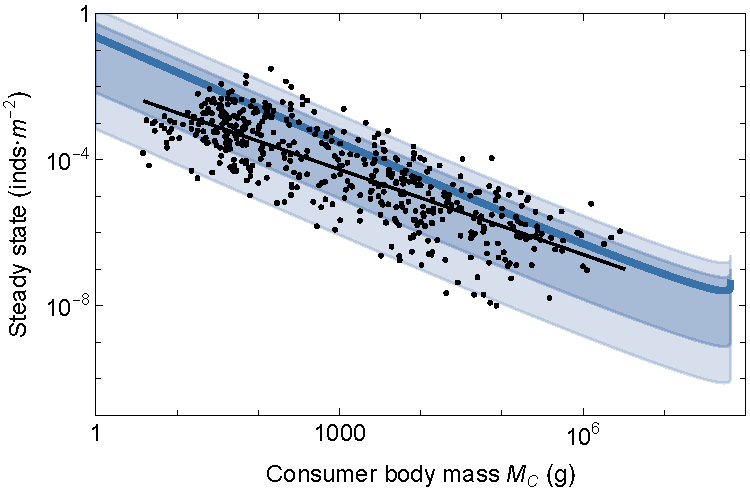
\includegraphics[width=0.5\textwidth]{fig_consumer2d_resources.pdf}
\caption{
\footnotesize
Model predictions of mammalian steady states compared to observational data from Damuth (REF).}
\label{fig:2ddensities}
\end{figure}



% \subsection{Starvation mortality (foundational, intrinsic, mass-specific, small-size punishing)}

% In the equilibrium scenario with starvation as the sole source of mortality, reproduction and mortality rates are equal for all consumer body-masses.
% As these rates are examined at the system equilibria this matching of rates is by definition and not ecologically interesting.

% How does starvation mortalty contribute to Damuth's Law?
% We assess the influence of each parameter in the model on 1) Damuth intercept and 2) Damuth slope
% We find:
% Non-allometric parameters (resource growth, carrying capacity) both influence intercept... Higher yield (grams consumer per gram of resource) increases overall steady states; higher starvation rates decrease overall steady states. This is all pretty intuitive
% Only allometric parameters influence the slope, as expected
% Higher growth rates of consumer lead to steeper slopes... this is the productivity paradox, but here we observe that this will more negatively impact larger consumers
% Increased yield (grams consumer per grams of resource) makes SLOPE shallower + INTERCEPT higher ~ high tides raise all ships
% increased maintenance rates make slope shallower without impacting intercept... benefiting the larger consumers, which take on higher steady states due to their increased efficiencies... i.e. larger consumers suffer less when maintenance becomes more costly, shallowing the slope
% increased starvation rates make slope shallower and lowers intercept -- similar to maintenance - while the effect overall is lower densities with higher starvation rates (intercept), larger organisms suffer less due to increased protection from starvation due to higher fat reserves.

At steady state, the allometric consumer-resource model provides an approximation to the mass-density relationship observed among terrestrial herbivorous mammals (REF). 
Importantly, the magnitude and slope of this approximation is a product of the vital rates in Eq. \ref{eq:2d} that are driven by both physiology and the environment, and it is useful to understand which components drive different aspects of the relationship.
To disentangle the influence of the various parameters in the consumer resource model, we evaluate the influence of a percent-change to each.
% as $\boldsymbol{\theta}(1 + \chi)$ where $\boldsymbol{\theta}$ represents the vector of parameters and $\chi$ is a random variable uniformally distributed between 0.5 and 1.5.
% By evaluating consumer steady states with randomly-generated error (5000 repetitions), we calculate the correlation between parameters $\boldsymbol{\theta}$ and the two principle components of Damuth's law: the mass-density intercept and the mass-density slope. 
The parameters influencing just the mass-density intercept are those that determine resource availability, including the resource's intrinsic growth rate $\alpha$ and carrying capacity $k$.
As the resource growth rate or carrying capacity are increased, so is the consumer's mass-density intercept.
An increase in the mass-density intercept means that the steady states of all consumer species -- irrespective of body size -- are raised, capturing the effects of higher productivity.
% This influence is clearly shown by Eq. \ref{eq:2dss} given that both $\alpha$ and $k$ reside solely in the numerator of $C^*$.

While our framework dictates that plant growth rates and carrying capacities are directly proportional to consumer steady states, we can gain insight into what drives the very large range of observed consumer densities by exploring the observed ranges of $\alpha$ and $k$ in terrestrial systems.
We assume an intrinsic growth rate roughly that of grass where $\alpha = 9.45\times 10^{-9}$ (s${}^{-1}$; REF), whereas observations among terrestrial plants reveal a range in growth rates from $2.81\times 10^{-10}$ to $2.19\times 10^{-8}$ \citep{michaletz2014convergence}, according with a change in $\alpha$ of roughly 97\% lower and 130\% higher than the set value. 
By incorporating this range into our the estimated resource growth rate, we observe that we can account for a large portion of consumer steady state densities around the mean density given by Eq. \ref{eq:2d} (inner shaded region, Fig. \ref{fig:2ddensities}).
If we additionally adjust the carrying capacity $k$ of the resource to 90\% less-than and 150\% more-than the assumed value of $23\times 10^3$ g/m${}^2$, our framework accounts for nearly the full range of mammalian steady state densities (outer shaded region, Fig. \ref{fig:2ddensities}).
In this context, the upper-boundary of $k$ observed to capture most higher herbivore densities is ca. 34 kg/m${}^2$, which is on the higher end of estimated live above-ground biomass densities in terrestrial forests such as in Isle Royal and the Allegheny National Forest \citep{de2017simulating}.
% With an energy density of ca. 5.77 kiloJoules/gram, higher than but within range of the carrying capacity of $664\times10^3$ kJ/m${}^2$, [within the range of possibility for terrestrial systems, REF].



\subsection*{Starvation and natural mortality disproportionately impact smaller consumers}

Considering how variations to the underlying energetic parameters driving consumer-resource dynamics alters the expected mass-density relationship may shed light on key constraints shaping mammalian communities. 
% PARAMETERS INFLUENCING INTERCEPT ONLY
Consumer growth rate $\lambda_C$, maintenance rate $\rho$, and yield $Y_C$ must vary widely from their expected value to have a measurable effect on the consumer mass-density relationship (Supplementary Fig. \ref{fig:corr}).
In contrast, variations to starvation-induced mortality have a large effect on consumer steady states, though the effect is not the same across body mass.
We introduce modifications to the rate of starvation as $\sigma^\prime = \sigma(1+\chi_s)$, where ${}^\prime$ denotes the modified rate and $\chi_s$ is the proportional change.
The relative change in the steady state introduced by the modified rate is then calculated as 
\begin{equation}
\frac{C^*(M_C|\sigma(1+\chi_s)) - C^*(M_C|\sigma)}{C^*(M_C|\sigma)},
\end{equation}
where higher values indicate a relative gain in steady state densities, and negative values indicate a relative loss (Fig. \ref{fig:starve}).
We observe that, while all mammals benefit from reduced starvation rates ($\chi_s<0$), smaller-bodied mammals benefit to a much greater extent, and this effect tapers off with increasing body mass.
% Changes to the starvation rate have a large effect on both the consumer-density intercept and slope (Fig. \ref{fig:corr}E,F).
% We observe that decreasing $\sigma$ from the expected value ($\chi<0$) serves to increase the steady state intercept, while decreasing the mass-density slope.
% By comparison, increasing $\sigma$ from the expected value ($\chi>0$) has less effect on the mass-density relationship.
% In the consumer-resource model described in Eq. \ref{eq:2d}, starvation is the sole source of consumer mortality, and therefore plays an out-sized role in determining consumer steady states. 
% As this mortality is reduced, consumer densities increase, raising the intercept.
% However, as consumer starvation rates decline we observe a steeper mass-density slope.
% Reduced starvation rates therefore principally benefit the steady state densities of smaller species, with reduced effects observed for larger-bodied mammals.
Because fat biomass scales super-linearly with body mass, the populations of larger consumers are thus more resilient to the effects of starvation, whereas those of smaller consumers are more prone.



\begin{figure}[h!]
    \centering
    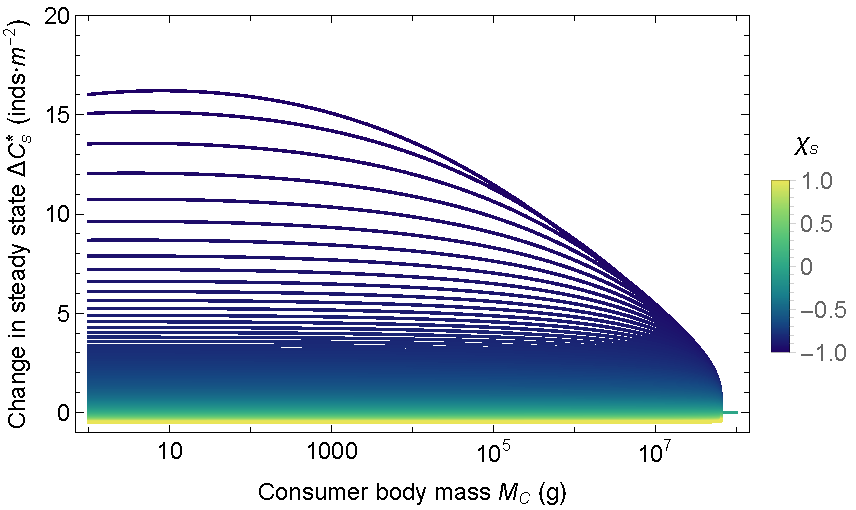
\includegraphics[width=0.5\textwidth]{fig_starverelative.pdf}
    \caption{
    \footnotesize
    Caption}
    \label{fig:starve}
\end{figure}



An organism's rate of starvation emerges from two governing forces -- the amount of energy storage and the rate of its use -- and as such can be be manipulated both physiologically and behaviorally.
For instance, behaviorally supplementing endogenous fat stores with exogenous caches magnifies an individual's energetic stores \citep{yeakel2020caching}, whereas physiologically-mediated responses to starvation risk such as torpor can introduce significant temporal delays to the effects of resource scarcity \citep{schubert2010daily}.
While these mechanisms are very different, in both cases the time required to pass from a replenished to a starved state is effectively increased, lowering the rate of starvation.
As shown in Fig. \ref{fig:corr}E,F, the predicted benefits of such adaptations to mammalian steady state densities will be realized primarily by smaller mammals, and it is these size classes where traits such as caching and torpor are most common \citep{geiser1998evolution,smith1984evolution,yeakel2020caching}. 
Additional sources of mortality may introduce very different effects on consumer populations, and we next explore how mortality beyond starvation informs our understanding of size-dependent extinction risks.
We next examine the effects of \emph{i}) initial cohort and actuarial mortality, \emph{ii}) mortality due to natural predation, and \emph{iii}) mortality due to external harvesting.

Importantly, changes to the starvation rate have a large effect on both the consumer-density intercept and slope (Fig. \ref{fig:corr}E,F).
We observe that decreasing $\sigma$ from the expected value ($\chi<0$) serves to increase the steady state intercept, while decreasing the mass-density slope.
By comparison, increasing $\sigma$ from the expected value ($\chi>0$) has less effect on the mass-density relationship.
In the consumer-resource model described in Eq. \ref{eq:2d}, starvation is the sole source of consumer mortality, and therefore plays an out-sized role in determining consumer steady states. 
As this mortality is reduced, consumer densities increase, raising the intercept.
However, as consumer starvation rates decline we observe a steeper mass-density slope.
Reduced starvation rates therefore principally benefit the steady state densities of smaller species, with reduced effects observed for larger-bodied mammals.
Because fat biomass scales super-linearly with body mass (see methods; REFS), the populations of larger consumers are more resilient to the effects of starvation, whereas those of smaller consumers are more prone.

An organism's rate of starvation emerges from two governing forces -- the amount of energy storage and the rate of its use -- and as such can be be manipulated both physiologically and behaviorally.
For instance, behaviorally supplementing endogenous fat stores with exogenous caches magnifies an individual's energetic stores \citep{yeakel2020caching}, whereas physiologically-mediated responses to starvation risk such as torpor can introduce significant temporal delays to the effects of resource scarcity \citep{schubert2010daily}.
While these mechanisms are very different, in both cases the time required to pass from a replenished to a starved state is effectively increased, lowering the rate of starvation.
As shown in Fig. \ref{fig:corr}E,F, the predicted benefits of such adaptations to mammalian steady state densities will be realized primarily by smaller mammals, and it is these size classes where traits such as caching and torpor are most common \citep{geiser1998evolution,smith1984evolution,yeakel2020caching}. 
Additional sources of mortality may introduce very different effects on consumer populations, and we next explore how mortality beyond starvation informs our understanding of size-dependent extinction risks.
We next examine the effects of \emph{i}) initial cohort and actuarial mortality, \emph{ii}) mortality due to natural predation, and \emph{iii}) mortality due to external harvesting.


% \subsection{Initial cohort and actuarial mortality disproportionately impact smaller consumers}
% \subsection{The Many Faces of Death} %This might be just for us ;)
% \subsubsection{Survivorship mortality (intrinsic, mass-specific, small-size punishing))}

% We consider three additional sources of mortality that are unrelated to starvation due to resource limitation: \emph{i}) initial cohort and actuarial mortality, \emph{ii}) mortality due to natural predation, and \emph{iii}) mortality due to external harvesting.
% Because these sources of mortality do not feed back to influence resource dynamics except through changes to consumer population densities, we leave the resource dynamic ${\rm d}R/{\rm d}t$ reported in Eq. \ref{eq:2d} unaltered and describe only alterations to the consumer equation.
%What is the rate of life history mortality?
Cohorts within populations experience two primary sources of natural mortality: the initial cohort mortality rate $q_0$ (${\rm s}^{-1}$) and the annual rate of increase in mortality as the cohort ages, or the actuarial aging rate, $q_a$ (${\rm s}^{-1}$) over lifetime $t_\ell$ (s).
We begin by assuming that the number of survivors over time follows a Gompertz relationship (see methods for details) from which we can derive the average rate of natural mortality \citep{CalderIII:1983jd,yeakel2018dynamics}
\begin{equation}
    \mu = \frac{q_0}{q_a t_\ell}\left({\rm e}^{q_a t_\ell}-1\right).
\end{equation}
% and where $\mu$ influences consumer population densities as
% \begin{equation}
%     \frac{{\rm d}}{{\rm d}t}C = \lambda^{\rm max}_{\rm C}RC- \left(\sigma \left(1 - \frac{R}{k}\right) + \mu \right)C.
% \end{equation}
The three parameters $(q_0,q_a,t_\ell)$ included in our description of natural mortality each have well-documented allometric relationships for terrestrial mammals (TABLE), such that natural mortality can be written as a function of consumer mass $\mu(M_C)$.
% such that $\mu$ follows an allometric scaling with exponent ca. -0.56.


\begin{figure}[h!]
    \centering
    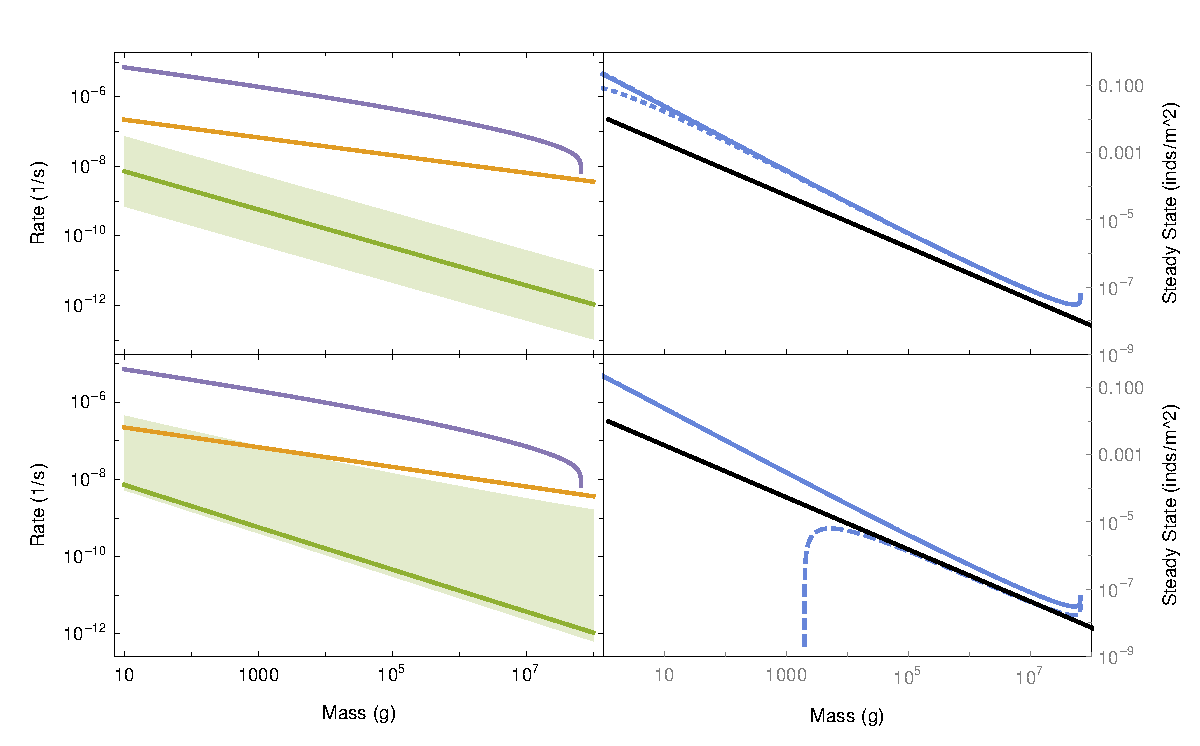
\includegraphics[width=0.9\textwidth]{joined_survivorship.pdf}
    \caption{
    \footnotesize
    Caption}
    \label{fig:naturalmort}
\end{figure}



We gain immediate insight into system constraints by examining how the rates of consumer mortality compare with consumer reproduction, with the expectation that stability requires mortality rates to be lower than reproduction (Fig. \ref{fig:naturalmort}A).
The starvation rate is a key exception, given that $\sigma$ represents the maximal rate of starvation whereas the effective rate is inversely proportional to resource density.
Because organisms can starve and recover many times over the course of their lifetime, the maximal rate of starvation $\sigma(M_C) > \lambda_C(M_C)$ over mass with the consumer steady state remaining stable.
We observe that survivorship mortality, including both initial cohort mortality and actuarial mortality, is both much lower and projects a steeper slope over $M_C$ than the rates of reproduction and starvation-induced mortality (Fig. \ref{fig:naturalmort}B), with an exponent ca. -0.56 \citep[cf.][]{jones2008senescence}.
While the calculated value of $\mu$ is nearly one order of magnitude below the rate of reproduction $\lambda_C$, a steeper slope implies that an overall increase in $\mu$ is expected to be more harmful to smaller organisms. 
While this relationship is well-known \citep{CalderIII:1983jd}, its predicted effects on consumer steady state have not been explored.


To understand the effect of variations in $\mu(M)$ on consumer steady state across body mass, we examine variations in the principle components of $\mu$: initial cohort mortality $q_0$ and actuarial mortality $q_a$.
%initial cohort mortality
The initial cohort mortality represents the mortality experienced by a cohort prior to the accruing effects of age. 
As $q_0$ is increased or decreased, the mortality rate changes in direct proportion, independent of consumer mass.
For survivorship mortality to approach the rate of reproduction, where perceptible declines in population densities result, the initial cohort mortality must increase by roughly an order of magnitude (shaded region in Fig. \ref{fig:naturalmort}A), and due to the steepness of $\mu$, this effect is felt exclusively by small-bodied organisms (Fig. \ref{fig:naturalmort}B).

%actuarial mortality
Actuarial mortality represents the cumulative effects of aging-induced mortality, or senescence, over the organism's expected lifetime. 
We observe that as $q_a$ increases, the magnitude of mortality rises while the slope of $\mu(M)$ becomes more shallow over $M$ (Fig. \ref{fig:naturalmort}C), primarily due to the cumulative nature of senescence magnifying its effects across the longer lifetimes of larger mammals.
As such, an order of magnitude increase overwhelms the reproduction of mammals up to ca. 1.2 Kg (Fig. \ref{fig:naturalmort}D), resulting in the destabilization of their respective populations. 
% Were an ecological context to arrive that dialed up the actuarial rate the community would be defaunated by size class from small to large.
The extinction risks imposed by senescence have been explored among a number of mammalian groups, where longer intervals between litters may promote declining population viability, while the influence of body size is less clear \citep{robert2015actuarial}.
Though our model -- which considers averaged effects across terrestrial mammals -- predicts that the most extreme risks imposed by increased actuarial mortality impacts smaller size-classes, we also show that $\mu$ increasingly resembles $\lambda_C$ with increasing $q_a$ (the top border of the shaded region in Fig. \ref{fig:naturalmort}C).
This increased similarity implies that relatively small variations in other demographic processes or interactions may have potentially large and destabilizing effects on population size.
We suggest that such effects may be a contributing factor to the noted ambiguity in the role of body size on increased rates of senescence across mammalian groups \citep{robert2015actuarial}.
% Our prediction of this increased similarity between reproductive and natural mortality rates across body size may be a contributing factor for the noted ambiguity in the effects of body size on increased rates of senescence across different mammalian groups \citep{robert2015actuarial}.


% [Body mass more complicated, but here we are looking at only terrestrial organisms]
% [taken across species and not including the details of life history, while our model forecasts population crashes for small-bodies species, the shallowing of $\mu$ with increasing actuarial mortality results in a very similar $\mu$ and $\lambda_C$ across $M$]
% [This means small variations in other life history variables may have unpredictable effects on population size]
% [explains some of the ambiguity in the effects of actuarial mortality as a function of body size.]



\subsection*{Predation mortality and the feasibility of megatrophic interactions}
% (extrinsic, mass-specific, small-size punishing)}

We next explore the effect of predator mortality on an herbivore consumer, taking into account carnivore-specific growth and energetic rates.
% Without explicitly taking into account the dynamics of a predator population, 
We account for the effects of an implicit predator density $P$ with body size $M_P$ on the herbivore consumer density $C$ with body size $M_C$.
% , where we will for now assume that the predator population exists at some steady state $P^*$.
% Using a form similar to consumer-resource consumption in Eq. \ref{eq:2d}, 
The mortality rate of the herbivore consumer from an external predator is then given by $\lambda_P(C) P/Y_P$, where $\lambda_P(C)$ is the growth rate of the predator and $Y_P$ is the predator yield coefficient, describing the grams of predator produced per gram of prey consumed (see methods).
% $C$, and $P$ is the density of the predator population.
% \begin{equation}
% \frac{{\rm d}}{{\rm d}t}C = \lambda^{\rm max}_{\rm C}RC- \left(\sigma \left(1 - \frac{R}{k}\right) + \mu + bP^* \right)C.
% \end{equation}
% The capture efficiency $b$ of the predator population describes the per-predator consumption rate of the herbivore prey $C$.
Assuming a linear functional response for predation mortality, $\lambda_P(C)$ is maximized when the consumer reaches its theoretical maximum population density, which we calculate by converting the resource carrying capacity directly to grams of consumer produced, or $C^{\rm max} = Y_C k$.
While this is an ultimately unattainable theoretical bound it allows for a direct calculation of the predator growth rate as a function of $C$, written as
\begin{equation}
    \lambda_P(C) = \lambda_P^{\rm max}\frac{C}{C^{\rm max}} = \lambda_P^{\rm max}\frac{C}{Y_C k},
    \label{eq:predfunction}
\end{equation}
where $\lambda_P^{\rm max}$ is the maximum predator growth rate (see methods). 
% assuming mammalian carnivore-specific metabolic relationships (see methods). 
% We assume that the predator capture efficiency is proportional to predator reproduction $\lambda^{\rm max}_P=\lambda_P/\hat{k}$, where the intrinsic reproductive rate $\lambda_P$ scales with maximal resource growth at one half resource carrying capacity $\hat{k}$.
% The capture efficiency can then be expressed as
% \begin{equation}
%     b = \frac{\lambda^{\rm max}_P}{Y_P Y_C},
%     % = \frac{\lambda_P}{Y_P(Y_C \hat{k})},
% \end{equation}
% where $Y_P$ is the predator yield coefficient describing the grams of predator produced per grams of herbivore prey consumed.
% Together, $Y_P Y_C$ thus represent the grams of predator produced per gram of resource consumed by its prey, mirroring our parameterization of the resource consumption rate in Eq. \ref{eq:2d}.
% Both the maximal rates of consumer growth $\lambda^{\rm max}_C$ and predator growth $\lambda^{\rm max}_P$ can be used to accurately predict the upper bounds of herbivore and carnivore population densities, respectively (see Supplementary Appendix XX), lending particular support for our scaling of maximal consumer and predator growth rates. 
% Finally, because we do not explicitely include the full dynamics of the predator population, we assume predators exist at empirically measured steady state densities, where that $P\equiv P^*\propto M_P^{-0.88}$ \citep{carbone2002common}.  
The theoretical boundary density for herbivore consumers $C^{\rm max}$ can similarly be used to calculate the boundary density for predators, $P^{\rm max} = Y_P C^{\rm max}$, both of which accurately capture the upper-bounds of herbivore and carnivore mass-density relationships (dashed lines in Fig. \ref{fig:predrate}A).
Because the effects of the predator are implicit, we assume that the predator population remains at empirically measured carnivore steady state densities, where $P\equiv P^*\propto M_P^{-0.88}$ \citep{carbone2002common}.  



% %Predation less than max
% Though we are not explicitly modeling the predator population, we expect the per-predator capture efficiency to decline as the consumer population is below a critical density.

% [We've thus scaled the intrinsic predator growth rate in the same way as consumer growth... to the maximal growth of resources]
% [This represents maximum predator growth]
% [We can check that this scaling makes sense -- predicts upper boundary of predator data]

% [We observe that $\lambda_P^{\rm max}$ is the reproductive rate of the predator population per gram of herbivore prey consumed.]
% In this case we define this critical point by the half-saturation density of resources $\hat{k}$, such that $\lambda_P^{\rm max} = \lambda_P/\hat{k}$ where $\lambda_P$ is the predator's intrinsic rate of increase, and $Y_C \hat{k}$ represents the grams of consumer produced under the conditions of maximum resource growth.
% % , such that $b = \lambda_P^{\rm max}/Y_P$. % , such that $\lambda_P^{\rm max} = \lambda_P/\hat{k}_C$
% % The predator yield coefficient scales proportionally with the individual mass of the predator and the energy density of prey, normalized to the lifetime energetic needs of a predator individual reaching maturity.

The predation mortality rate depends on both the body size of the herbivore consumer and its respective predator. 
% The predator yield coefficient scales proportionately with predator body size and the energy density of its prey $E_C$, such that $Y_P \propto M_P E_C$.
% Because we are assuming that the predator population is external to our consumer-resource model, the mortality rate experienced by the herbivore population $bP$ is sensitive to predator size in two ways: \emph{i}) larger predator body sizes will increase the predator yield, lowering the attack efficiency
Trophic interactions are constrained by body size \citep{Sinclair2003,Brose2005,Hatton:2015fk}, and large prey generally suffer mortality from large predators, though the nature of predator-prey mass ratios (PPMRs) varies across communities \citep{barnes2010global}, organismal body size \citep{Brose2005,Rohr2010,Yeakel2014,pires2015pleistocene}, and is not well understood outside of aquatic gape-limited systems \citep{nakazawa2017individual}.
% Because our framework is herbivore-centric, we require a prediction of the expected predator mass given an herbivore of body size $M_C$.
Using dietary information for larger predators and prey ($>10^5$ g) \citep{Hayward2005,Hayward2006,Hayward2008}, the expected carnivore mass given a particular herbivore mass follows roughly ${\rm E}(M_P|M_C) = p_0 M_C^{p_1}$, where $p_0 = 11786.8$ g and $p_1 = 0.194$ (Supplementary Fig. \ref{fig:ppmr}). %A) Hayward replicated data; B) pred size per herb size
Unlike marine systems, larger terrestrial herbivores tend to suffer mortality from smaller predators, an asymmetry that becomes more pronounced with increasing size \citep[cf. ][]{Sinclair2003}.
We note that smaller predator/prey size classes tend to follow different PPMR relationships, where predators tend to be much larger than prey (e.g. rodent- or insect-specialist mesocarnivores) \citep{cruz2022geography,Cruz2022}.
% , so we limit our current analysis to those occupying size classes $\geq 100$ Kg.


% To assess the effects of predation as a function of herbivore consumer mass, we must establish a predator size-scaling, so that a consumer with mass $M_C$ is assumed to be the focal prey of a predator with size $M_P(M_C)$.
% Using the logit framework introduced by Rohr et al. \citep{Rohr2010} to predict the probability of a trophic interaction between two species as a function of predator to prey body size ratios, the mean predator body size for a prey of mass $M_C$ is given by $M_P = M_C{\rm exp}(\frac{p_1}{2p_2})$, where $p_1$ and $p_2$ are parameters with values fit to the adjacency matrix of a known food web.
% To capture terrestrial mammalian predator-prey relationships we use fittings derived for the mammalian Serengeti food web \citep{Yeakel2014,pires2015pleistocene}, resulting in $M_P(M_C) \approx (3/4) M_C$, where predator body size is smaller than that of prey. %such that $p_1 = 0.21$ and $p_2 = -0.37$, $
% We note that this particular parameterization is relevant primarily for larger predator-prey relationships, and we here limit our interpretation to larger size-classes.

% Because these relationships are system-dependent, we assume a predator body size scaling that is representative of the contemporary Serengeti, where on average 


% [EXPLAIN BRIEFLY WHAT GOES INTO b AND P]
% 1) The scaling of predator mass with increasing consumer mass
% 2) The assumption of an extrinsic predator existing at P^* \propto M_p^{-0.88}



% Even without exploring directly the consumer-resource dynamics, we can gain insight into the potential effects of predation mortality by comparing the mortality rate to the consumer's population growth rate $\lambda_C$ as a function of consumer mass $M_C$.
% While the consumer's reproduction rate scales $\lambda_C \propto M^{-0.25}$, the predation mortality rate is shown to scale $bP^* \propto M^{0.37}$, meaning there is a consumer mass $M_C$ where these rates intersect.
% For smaller consumer masses, the predation mortality rate is lower than the consumer's reproductive rate, suggesting that these populations can sustain a predator population.
% However, as consumer mass increases, the predation mortality rate crosses $\lambda_C$, at which point the predation mortality rate becomes larger than the consumer reproductive rate.
% This suggests that, given the optimal predator:prey mass scaling observed in diverse terrestrial communities (Eq. \ref{eq:opt}), there is a consumer mass threshold $M_C^{\rm crit}$ above which the consumer population can no longer sustain itself in the presence of such predative load.

% We can gain insight into the potential effects of predation mortality by comparing the mortality rate to the consumer's population growth rate $\lambda_C$ as a function of consumer mass $M_C$.
% As consumer mass increases, the predation mortality rate crosses $\lambda_C$, at which point the predation mortality rate becomes larger than the consumer reproductive rate.
% This suggests that, given the optimal predator:prey mass scaling observed in diverse terrestrial communities (Eq. \ref{eq:opt}), there is a consumer mass threshold $M_C^{\rm crit}$ above which the consumer population can no longer sustain itself in the presence of such predative load.
% While the analytical expression of $bP^*$ is not tractable, numerical assessment of this critical consumer mass gives $M_C^{\rm crit} = 1064$ Kg. 
% Our analysis suggests that a consumer mass above this threshold cannot sustain a predator population with a predator:prey mass ratio observed for lower body masses, and with densities predicted by Damuth's Law.
% Intriguingly, this corresponds to the body size of herbivores in the Serengeti that effectively escape predation due to their large size.
% Cape buffalo have a mass $M_C \approx 450$ Kg, where predation accounts for roughly $23\%$ of mortality, whereas giraffes with  mass $M_C \approx 800$ Kg suffer $\approx 5\%$ mortality due to predation.
% The next largest herbivore in the Serengeti are rhinoceros, which weigh $\approx 1200$ Kg and suffer $0 \%$ mortality due to predation (Sinclair et al.  2003), a threshold remarkably consistent with our estimated $M_C^{\rm crit}$ of 1064 Kg.


\begin{figure}[H]
  \centering
  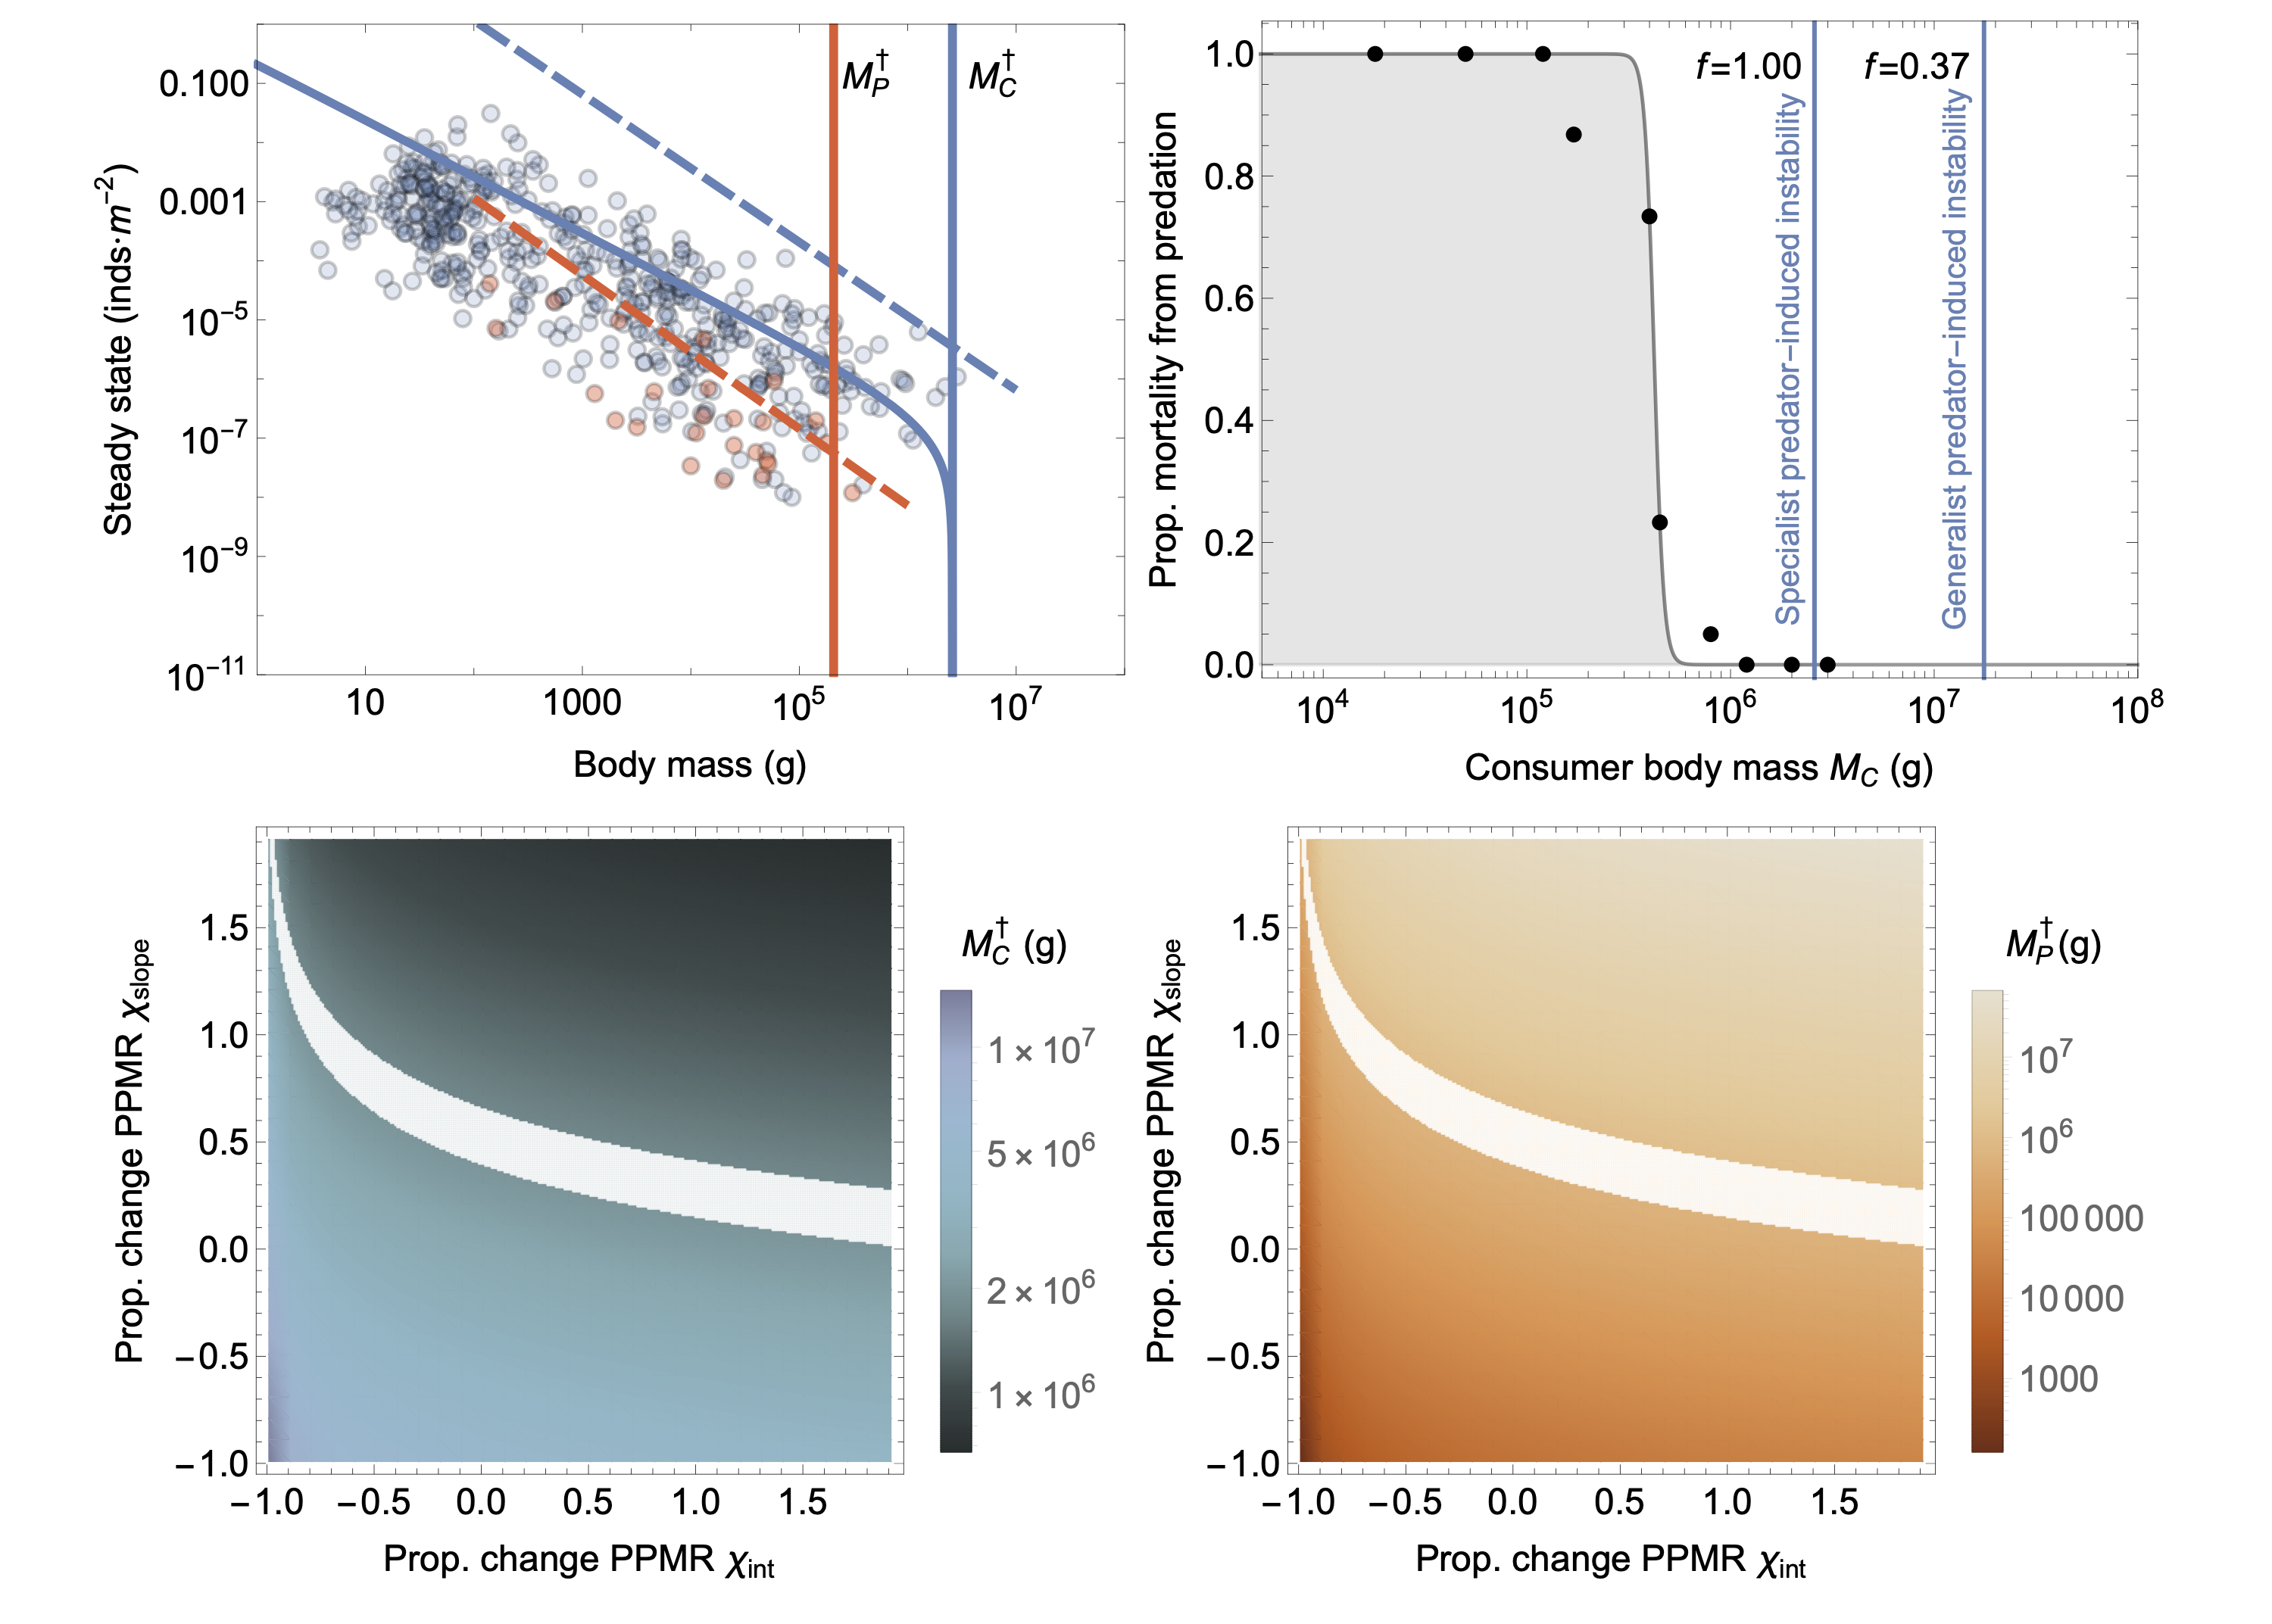
\includegraphics[width=0.8\textwidth]{fig_predation_alltogether.png}
  \caption{
  \footnotesize
	  A) Empirical mammalian herbivore (blue points) and predator (red points) mass-densities shown alongside the theoretical maximum herbivore $C^{\rm max}$ and predator $P^{\rm max}$ densities as a function of body size. 
	  The solid blue curve denotes the predicted herbivore consumer steady state $C^*(M_C)$ with predation mortality.
	  Predicted herbivore $M_C^\dagger$ and predator $M_P^\dagger$ size thresholds (blue and red vertical lines, respectively) reveal where the herbivore consumer population is no longer able to support a predator population. 
	  The blue shaded region denotes `mega' size classes $>1\times10^5$ g.
	  B) Percent mortality from predation for Serengeti herbivores (redrawn from Sinclair et al. \citep{Sinclair2003}) as a function of body mass $M_C$. Gray shaded region denotes a sigmoidal fit to the data with the inflection at $4.22\times10^5$ g. Vertical lines show herbivore size threshold under the assumption of predator specialization ($f=1.00$; $M_C^\dagger=2.58\times10^6$) and generalization ($f=0.37$; $M_C^\dagger=1.75\times10^7$).
	  C) Threshold herbivore sizes $M_C^\dagger$ across changes to the predator-prey mass ratio (PPMR) intercept and slope (see Eq. \ref{eq:ppmr}).
	  White shaded region denotes megatrophic threshold sizes, where both $(M_C^\dagger,M_P^\dagger) > 6\times10^5$ g. 
	  D) As in C), but showing the corresponding threshold carnivore sizes $M_P^\dagger$.
  }
  \label{fig:predrate}
\end{figure}


%The critical consumer mass MCdagger
Integrating the large-bodied PPMR relationship into the predation mortality rate reveals the emergence of a dynamic instability at megaherbivore size classes (Fig. \ref{fig:predrate}A), where here and throughout the prefix `mega' is used to signify size classes $>6\times10^5$ g \citep{Hayward2005}.
An implicit predator population with body size ${\rm E}(M_P|M_C)$ is thus able to withdraw sufficient biomass from an herbivore prey population to sustain itself for herbivore sizes lower than a threshold consumer body mass $M_C^\dagger = 2.58\times 10^6$ g (Fig. \ref{fig:predrate}A).
Above this critical size threshold, the herbivore population has such low densities that it is unable to sustain a predator species large enough to consume it, introducing a strong upper-bound to mammalian carnivore body size driven by a trophic cascade.
This boundary matches the herbivore maximum size limit observed in contemporary terrestrial systems, at roughly the size of an elephant \citep{Sinclair2003} (Fig. \ref{fig:predrate}B).
% While the largest herbivores do not suffer significant mortality from predation in contemporary ecosystems, this boundary is critical because it signifies the threshold where excess mortality renders the population highly unstable.
% The herbivore mass threshold is not incredibly sensitive to variation, where a $\pm 10\%$ change in mortality rates results in a $M_C^\dagger$ ranging from $2.15$ to $3.16\times10^6$ g (Supplemental Fig. XX), well within the elephant body mass range \citep{christiansen2004body}. %CHECK



While $M_C^\dagger$ marks the threshold herbivore mass above which predation is unsustainable, Sinclair et al. \citep{Sinclair2003} have shown contemporary herbivores to begin to escape predation at ca. $4.22\times10^5$ g (redrawn in Fig. \ref{fig:predrate}B).
This change-point reflects the limitations of contemporary carnivores, which reach a maximum body size of $1.15$ to $2.60\times10^5$ g \citep{Sinclair2003,Hayward2005}, and reveal preferences for prey up to $5.50\times10^5$ g \citep{Hayward2005}.
As such, the sole predators of contemporary giants are not megaherbivore specialists, instead opportunistically subsidizing their preferred prey base. %, while relying on a much smaller prey base.
% This highlights an important constraint of our framework: that predation suffered by the herbivore is exclusive to a single predator population, and that the single predator population is relying exclusively on a single prey.
While our framework assumes a specialized predator-prey interaction, the largest predators in natural systems tend be dietary generalists \citep{Sinclair2003}.
% In diverse mammalian communities, the largest predators also exhibit the largest prey size range \citep{Sinclair2003}, suggesting that only a fraction of predator biomass is expected to be supported by a single prey population.
We can introduce the effects of generalist predation by modifying the fraction of predator growth $f$ supported by the herbivore prey, such that the demands of predator growth are modified as $f\lambda_P(C)$.
% to a fraction of its current estimate, effectively simulating the influence of a generalist predator population.
We observe that increasing the implicit dietary generality of the predator increases $M_C^\dagger$ to a larger threshold mass.
For example, $f=0.37$ means that a predator is supporting a little more than 1/3 of its growth rate by the targeted prey, which increases the herbivore body mass boundary to $M_C^\dagger = 1.75\times10^7$ grams (Fig. \ref{fig:predrate}B; Supplemental Figs. \ref{fig:maxpreyvar},\ref{fig:megamammal}), roughly the body mass attained by the largest terrestrial herbivores, the late Eocene indricotheres and mid-Miocene deinotheres \citep{Smith:2010p3442,yeakel2018dynamics}.
That the threshold herbivore mass decreases with increasing predator specialization both emphasizes that larger predators are dynamically constrained to be dietary generalists citecite{Sinclair2003}, while also pointing to a positive feedback mechanism that may operate in systems undergoing megafaunal extinctions.
As megaherbivore species are lost, the largest predators must respond by increasing their reliance on those remaining.
Our results reveal that this energetic redirection will reduce the threshold herbivore mass $M_C^\dagger$ to lower size classes, thereby promoting additional extinctions and attendant predator specialization.



%NOTE: THE THRESHOLD IS ALWAYS AT LARGER SIZES

%RELAXING THE PPMR
% Contemporary megaherbivores do not represent the largest mammalian size classes ($>3\times10^6$ to $1.74\times10^7$ g), and there are no contemporary megapredators.
While deinotheres and indricotheres top the megaherbivore scale, the Eocene artiodactyl \emph{Andrewsarchus} may have been the largest terrestrial mammalian predator at $8\times10^5$ to $1\times10^6$ g (REF), while the Miocene Hyaenodontid \emph{Megistotherium osteothlastes} ranged between $5$ to $8\times10^5$ g \citep{sorkin2008biomechanical} and the early Eocene Oxyaenodont \emph{Sarkastodon mongoliensis} weighed ca. $8\times10^5$ g. %(Rasmussin 1989, Sorkin 2008)
% a recent skull of \emph{Smilodon populator} indicates that some individuals may have attained body sizes up to 900 Kg (REF).
A theoretical maximum mammalian carnivore size of $1.1\times10^6$ g has been proposed based on the intersection of daily energetic uptake requirements against metabolic expenditures \citep{Carbone:2007dz}, closely aligning with the largest known megapredators.
While our consumer-resource framework provides a range of predicted megaherbivore body mass thresholds depending on the fraction of predator growth it fuels, we next ask under what conditions megatrophic relationships between megaherbivores and megapredators are dynamically feasible.


A principle relationship in our framework is the allometric PPMR observed for the largest contemporary herbivores and carnivores, however it is not known whether this PPMR is representative of past megatrophic relationships.
In fact, it is likely that the contemporary PPMR does not account for these interactions, as deinotherium-sized herbivores result in ${\rm E}(M_P|M_C)=2.99\times10^5$ g, whereas the maximum carnivore body mass is $2-3\times$ larger.
While it is unknown whether these super-sized carnivores were specialists on deinothere size-classes (REFS), our framework allows us to investigate whether and to what extent changes to the contemporary PPMR enable megatrophic interactions, where we allow the PPMR to vary as 
\begin{equation}
{\rm E}(M_P|M_C) = p_0(1+\chi_{\rm int}) M_C^{p_1(1+\chi_{\rm slope})},
\label{eq:ppmr}
\end{equation}
where the proportional changes in the PPMR intercept and slope are given by $\chi_{\rm int}$ and $\chi_{\rm slope} \in (-0.99,2)$.
We find that the threshold herbivore body size $M_C^\dagger$ increases, while $M_P^\dagger$ decreases, with lower PPMR intercepts and shallower slopes (Fig. \ref{fig:predrate}C,D). %, whereas the threshold carnivore body size $M_P^\dagger$ decreases with the same 
Lower PPMR intercepts and shallower slopes mean that predator sizes are generally smaller, and increase more slowly, with larger herbivore body sizes.
So given a particular herbivore size, proportionately smaller predators elevate the threshold herbivore mass, while larger predators drive down the threshold herbivore mass.
% whereas smaller-bodied predators serve to elevate $M_C^\dagger$.
Importantly, only a small range of values for PPMR intercepts and slopes permit the existence of megatrophic interactions, with megaherbivore sizes spanning $1.72$ to $2.01\times10^6$ g and megapredator sizes spanning $6.11$ to $1.19\times10^5$ g (white band in Fig. \ref{fig:predrate}C,D).
While significantly larger PPMR intercepts are unlikely to be realized in natural systems, the megainteraction range does include very low intercepts combined with very high slopes, such that predator-prey ratios are low at smaller masses, and much higher at large body masses (Supplementary Fig. \ref{fig:ppmr}).
Such an hypothesized PPMR does not stray far from contemporary large-mammal interactions and may be a good candidate for megatrophic interactions. 

Feasible megatrophic interactions increase substantially if a smaller percentage of the predator growth rate is fueled by the target herbivore population ($f<1$).
Setting $f=0.37$ -- which we observed increases $M_C^\dagger$ to deinothere/indricothere size classes -- and allowing both $\chi_{\rm int}$ and $\chi_{\rm slope}$ to vary, results in megatrophic interactions spanning the largest megaherbivore ($1.27$ to $1.48\times10^7$ g) and megapredator ($6.15$ to $1.20\times10^6$ g) sizes observed in the fossil record (Supplementary Fig. \ref{fig:megamammalgen}).
% These results indicate that existence of megapredators in terrestrial systems requires generalist dietary behaviors, and only steeper PPMRs than those observed in contemporary systems enable interactions of the largest mammalian size classes.
% However, as ever-increasing predator body sizes may expand the size range of available herbivore prey, the increased demands of these predator populations lower the maximum sustainable herbivore body size.
% The sensitivity of this instability suggests that 
Our framework thus highlights dynamic constraints existing between predators and prey that may serve to structure terrestrial mammalian communities over evolutionary time, in particular revealing the tenuous positions of mega-sized herbivores and predators.
As carnivorous clades acquire body sizes enabling megaherbivore predation over evolutionary time, their super-sized appetites result in unsustainable megaherbivore densities where the risk of extinction becomes overwhelming -- an evolutionary trap marking the final tooth in the hypercarnivore ratchet \citep[cf.][]{VanValkenburgh:2004p2451}.
% While megapredators were unlikely to have been megaherbivore generalists, early human populations are known to have relied extensively on large-bodied species, and we next examine how our framework can be used to understand the effects of subsidized harvesting, potentially offering insight into the Pleistocene megafaunal extinctions.

% Carbone et al. \citep{Carbone:2007dz} have previously shown that a maximum carnivore size of 1100 Kg can be predicted from the intersection of daily energetic uptake requirements against metabolic expenditures.
% We can assess directly whether our estimate of $M_C^\dagger$ relates to an observed carnivore size threshold by calculating the expected predator size from our fitted relationship for $M_P(M_C^\dagger)$, which gives $M_P^\dagger = 1270$ Kg.
% As our predicted allometric predator mortal





% At these sizes, megaherbivores ($M_C > 1000$ Kg) only rarely suffer predation by the largest mammalian carnivores \citep{john2009lion,le2018megaherbivores}.
% The instability predicted by our framework at $M_C = M_C^\dagger$ suggests that as large-bodied carnivore clades increase in size over evolutionary time, they will tend to push their prey resources towards extinction -- an evolutionary trap marking the last tooth in the mammalian hypercarnivore ratchet \citep[cf.][]{VanValkenburgh:2004p2451}.




% Carbone et al. \citep{Carbone:2007dz} have previously shown that a maximum carnivore size of 1100 Kg can be predicted from the intersection of daily energetic uptake requirements against metabolic expenditures.
% We can assess directly whether our estimate of $M_C^\dagger$ relates to an observed carnivore size threshold by calculating the expected predator size from our fitted relationship for $M_P(M_C^\dagger)$, which gives $M_P^\dagger = 1270$ Kg.
% % As our predicted allometric predator mortality rate crosses the consumer's reproductive rate at $M_C^{\rm crit}$, the populations of herbivore speciers larger than $1064$ Kg are expected to collapse, an effect that would be expected to cascade into the predator population.
% % Because we assume that predator mass is dependent on prey mass, we can estimate the predator mass that would destabilize its prey population, for which we obtain $M_P^{\rm crit} = 802$ Kg.
% Our estimate of $M_P^\dagger$ corresponds closely to the largest observed terrestrial apex carnivores: the Hyaenodontid \emph{Megistotherium osteothlastes} ranged between 500-800 Kg \citep{sorkin2008biomechanical}, while the Oxyaenodont \emph{Sarkastodon mongoliensis} weighted $\approx 800$ Kg. %(Rasmussin 1989, Sorkin 2008)
% The artiodactyl \emph{Andrewsarchus} may have been the largest terrestrial predator at $800-1000$ Kg (REF), while a recent skull of \emph{Smilodon populator} indicates that some individuals may have attained body sizes up to 900 Kg (REF).
% These results provide an added perspective to Carbone et al.'s \citep{Carbone:2007dz} energetic threshold: that carnivore body size may additionally be limited by instabilities introduced to the populations larger body-sized herbivores.
% % [trophic allometry convergence by ]
% That multiple allometric constraints may converge around observed size thresholds has been noted before \citep{yeakel2018dynamics}, though is not well understood and may be a fruitful avenue for future efforts.

%pred/prey mass scaling
% We have assumed that the optimal mass ratio between predators and prey follows the scaling observed in the Serengeti food web, where $M_P/M_C \approx 3/4$ \citep{Yeakel2014,pires2015pleistocene}.
% While the plasticity of this relationship is difficult to examine for larger terrestrial carnivores given there are so few systems with diverse large-bodied carnivore guilds, recent efforts has revealed high plasticity among smaller carnivore taxa, as well as strong phylogenetic effects \citep{cruz2022geography}.
% For example, in marine systems predators are largely gape-limited (REF) such that the optimal mass ratio is roughly $XX$ where predators tend to be much larger than their prey, and this distinction from terrestrial systems points to substantial ecological variability across systems.
% By altering the assumed $M_P/M_C$ within our framework, we can examine directly how such trophic allometry impacts predicted herbivore population thresholds $M_C^\dagger$.










% [Because our framework is constructed based on underlying energetic relationships, we can now ask: how do variations in less constrained model parameters alter these estimated mass thresholds?]
%We observe that the predicted thresholds are very sensitive to changes in the energy density of the consumer population.
%The above conditions assume reported energy densities of protein and fat, and that the consumable portion of the prey has a protein:fat ratio of $\approx 32:68$.
%If, however, the J/g of fat within consumable tissue is increased, so does its energy density, which would be the case for prey such as marine mammals.
%For example, if the J/g of fat within consumable tissue is increased by 5\%, we observe the threshold predator body size to increase to 795 Kg; if the J/g of fat is increased by 10\%, threshold predator mass increases to 1000 Kg.
%While we do not examine specifically the changed conditions of prey within maritime environments, the largest terrestrial carnivore \emph{Ursus maritimus} maintains a diet composed of the energy-rich marine mammals.
%The directionality of our model predictions thus affirms expectations of larger maximimum carnivore mass conditioned on a diet composed of prey with tissues that have greater energy density.
% [Pleistocene implications]




\subsubsection*{Harvesting to extinction} 
% (extrinsic, mass-non-specific, large-size punishing)}

We last consider the effects of anthropogenic harvest-induced mortality on consumer populations.
While the predation rate is naturally limited by the energetic needs of the predator, we consider harvest to be a comparatively unconstrained source of mortality.
This may be the case if the human population(s) engaged in harvesting are subsidized by alternative resources (Brook 2005).
Harvest pressure has potentially varying relationships with consumer (prey) body mass, a complex product of environment, climate, culture, and technology (REFS), where harvest rate $h(M_C) = \xi M_C^\ell$.
For example, hunting traditions specializing on mass-collecting, by way of trapping or netting (Churchill 1993; Ugan 2005) are expected to exhibit harvest allometries biased towards smaller species (negative size-scaling, $\ell<0$), whereas a purely opportunistic strategy may be expected to have very little allometric dependence (zero size-scaling, $\ell=0$).
Inclusion of negative size-scaling harvest reveals that smaller-sized prey can withstand significant harvesting pressure before their populations are negatively impacted.
While smaller mammals do not appear to offer a significant return on investment (though see Hudson et al. 2019), the mass-collecting of invertebrates such as grasshoppers, and fish can offer significant returns (Ugan 2005).
In contrast, the inclusion of zero size-scaling harvest reveals that it is the larger-bodied organisms that are negatively impacted, but only if $h(M_C) > \lambda_C(M_C)$ (Supp. Fig. \ref{fig:harvestscaling}).



\begin{figure}[h!]
    \centering
    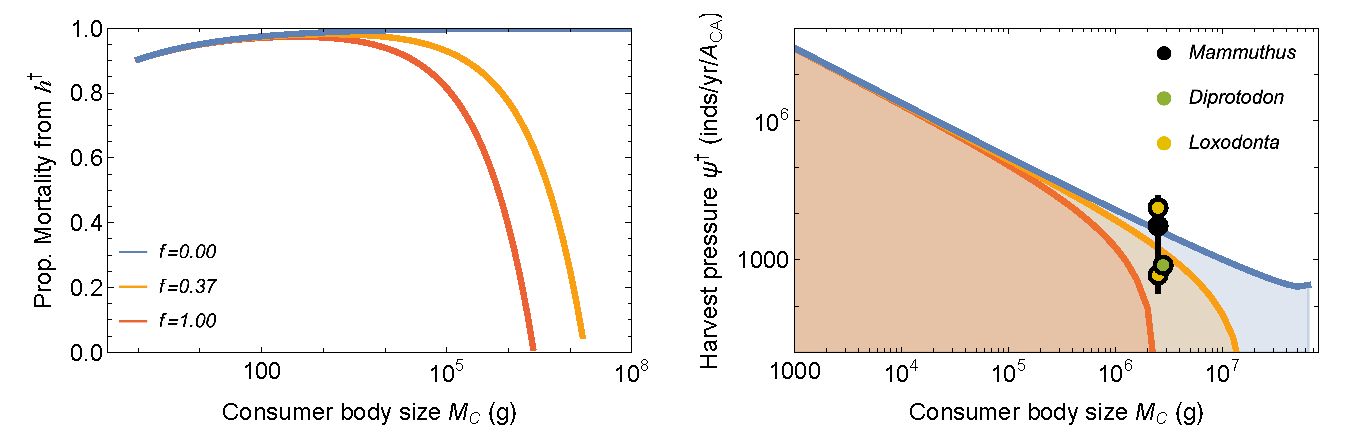
\includegraphics[width=1\textwidth]{fig_harvest.pdf}
    \caption{
    \footnotesize
    A)  
    }
    \label{fig:harvest}
\end{figure}



Technology provides access to otherwise unobtainable size-classes of potential prey, and is expected to strongly influence the allometry of harvesting effort.
% In contrast to these hypothetical harvest relationships, 
For example, the innovation of advanced projectiles is thought to have enabled harvest of terrestrial megafauna (Churchill 1993; Prates 2022), while archeological evidence points to many Pleistocene human populations as potential megafaunal specialists (positive size-scaling, $\ell > 0$; Broughton 2011; Lyons et al. 2016).
% , switching to sub-mega size classes with the decline of megafaunal diversity (Buchanon et al. 2011).
More recently, historical fisheries have been subject to positive size-scaling harvest efforts (Sethi et al. 2010), and contemporary size classes may be much reduced due to the accumulation of these pressures over time (Jennings 2004).
While the allometry of harvest effort is largely unknown (REF) and highly plastic (REF), our framework allows us to examine how much effort is required to induce population collapse as a function of mammalian body size. % -- regardless of harvest scaling --


We next calculate the harvest rate required to induce extinction, $\xi^\dagger$, as a function of body size $M_C$, and find a scaling relationship proportional to the mass-density relationship where $\xi^\dagger \propto M_C^{-1/4}$.
% We denote the harvest rate sufficient 
This is a natural result, as the effort required to suppress a population is expected to be proportional to the consumer's abundance. 
As a proportion of the other sources of consumer mortality that we have considered excluding predation ($f=0$), extinction-level harvesting is lower for smaller consumers, saturating at close to unity for larger consumers, reflecting the role of starvation mortality among small-sized organisms with lower proportions body fat.
With predation mortality included at both generalist ($f = 0.37$) and specialist levels ($f=1$), extinction-level harvesting accounts for an increasingly smaller proportion of mortality for larger organisms (orange and red lines, Fig. \ref{fig:harvest}A).
This relationship highlights the delicate nature of the megafaunal niche, where smaller changes in mortality rates can induce population collapse.

To examine how our estimate of extinction-level harvesting rates $\xi^\dagger$ compare to those estimated for human hunting of paleontological and historical mammalian populations, we converted $\xi^\dagger$ to harvest pressure, $\psi^\dagger$, or the number of individuals harvested per year to reduce the population to a fraction of its steady state $\epsilon C^*$ where we set $\epsilon = 0.01$.
We calculate $\psi^\dagger$ for an arbitrary area, which we standardize as the area of California ($A_{\rm CA} = 4.24\times10^5~{\rm km}^2$), such that
\begin{equation}
    \psi^\dagger \propto -\xi^\dagger\frac{C^*(1-\epsilon)}{M_C \log(\epsilon)}.
\end{equation}
This estimate of harvest pressure, while assuming a constant depletion from the population steady state such that it is conservative on greater-than-generational timescales (see Supplemental Materials XX), also permits direct comparison to other published estimates.
We observe that -- though the annual harvesting pressure is unrealistically high for smaller organisms -- it is ca. $1.2\times10^4~{\rm inds/yr/}A_{\rm CA}$ for organisms $>10^6$ g in the absence of predation mortality ($f=0$).
With the increasing pressures of generalist and specialist predation, the harvest pressure required to induce extinction is much less for larger consumers (Fig. \ref{fig:harvest}B).
% , and $>1.8\times10^6$ g in the presence of predation mortality (Fig. \ref{fig:harvest}B).

Our predictions of extinction-inducing harvest pressure compare well with historical and paleontological estimates of harvesting pressure on mammalian megafauna. 
For example, Fordham et al.'s (2021) estimate of the harvesting pressure required to collapse mammoth (\emph{Mammuthus primigenius}) populations (using a formulation similar to that of Alroy; 2001) revealed a range of values consistent with our expectation for similar size-classes (est. harvest pressure = $5.37\times10^4~{\rm inds/yr/}A_{\rm CA}$), as did estimates for the Australian \emph{Diprotodon} (est. harvest pressure = ca. 763 ${\rm inds/yr/}A_{\rm CA}$; Bradshaw et al. 2021).
Within the historical record, elephant populations experienced comparatively lower harvest pressure through 1850 (ca. 466  ${\rm inds/yr/}A_{\rm CA}$), a value derived from the volume of ivory exports (Milner-Gulland 1993), scaled to African elephant habitat area ($3.22\times 10^{6}~{\rm km}^2$; Thouless, 2016).
While fluctuating over the next century, harvest pressure elevated to a maximum of ca. $13.3\times 10^5~{\rm inds/yr/}A_{\rm CA}$ just prior to 1987 (Fig. \ref{fig:harvest}B).
This level of harvest was not sustained, as ivory export volume plummeted following the implementation of trade restrictions in 1989 (Milner-Gulland 1993).
% While this level of harvest is greater than our estimate to induce population collapse (Fig. \ref{fig:harvest}B), it was not sustained, as ivory export volume plummeted following the implementation of trade restrictions in 1989 (Milner-Gulland 1993).
Both Fordham et al.'s estimate for Pleistocene mammoths and the short-lived harvest maximum for African elephants in 1987 achieved levels greater than $\psi^\cross$ under the conservative assumption of zero natural predation pressure.
While estimates for $\emph{Diprotodon}$ harvest are considerably lower (Bradshaw et al. 2021), it is important to note that our measure of harvest pressure is parameterized for eutherian rather than marsupial mammals.
Nevertheless, the estimated \emph{Diprotodon} $\psi^\dagger$ is well within range of extinction-inducing harvest rates if natural predation pressures are also included, and there is evidence to suggest that \emph{Diprotodon} likely served as prey for marsupial lions (Runnegar 1981; Horton 1981; Wroe et al. 1999), and both giant crocodylians (\emph{Pallimnarchus}) and varanid lizards (\emph{Megalania}; Webb 2009).
% though these estimates must be viewed as lower-bounds given they are derived from ivory exports extracted from an unknown area, though standardized Africa, much larger than the area being harvested.




\section*{Conclusion}
We have shown that the inclusion of mass-specific energetic transfer between resources and consumers, combined with the unique timescales governing consumer mortality, both predict the observed mass-density relationship observed for mammals \citep{Damuth1987} and provide insight into dynamic thresholds constraining populations.
Both starvation and cohort mortality primarily impact small-bodied species, whereas the effects of increased senescence to scale similarly with consumer reproduction, potentially explaining the apparent lack of relationship between senescence and body size in natural systems.
On the other hand, we find that trophic mortality primarily impacts large-bodied species due to smaller population densities and longer generation timescales.
While this general relationship has been investigated in prior efforts (REF), we show that predation mortality induces dynamic thresholds on consumer body size, where both predator specialization and relative body size determines whether mega size classes are feasible.
The effects of predation stand in contrast to those of subsidized harvest, where we compare the mass-specific harvest pressure needed to induce extinction against estimates from the end-Pleistocene as well as the historical ivory trade.

Missing megafauna - herbivores and predators
Predators are constrained by their food... and large sizes are delicately balanced
House of cards plays into the ephemeral nature of these species
In particular their sensitivity to a subsidized harvesting pressure
But the benefits to largess ensure that the void is quickly filled
Our framework is minimal - few assumptions other than energetics
May offer insight into the primary constraints directing the composition of communities both past, present, future.




% We have shown that
% Timescales + LV fits Damuth
% Considering sources of mortality reveals differential impacts on small vs. large-bodied populations
% Observe dynamic thresholding emerging with the inclusion of predation mortality
% Exploration of potential changes into known predator-prey scaling reveals stability thresholds for megatrophic interactions
% Extinction inducing harvest rates are in line with expectations from past extinction events, as well as recent harvesting pressure on existing megafauna.

Where have all the megafauna gone? 
Allometric relationships principled on energetic dynamics scaled to population-level processes provides tools to investigate the gaps in our contemporary mammalian communities.


%%%%%%%%%%%%%%%%%%%%%
% Acknowledgments
%%%%%%%%%%%%%%%%%%%%%
% You may wish to remove the Acknowledgments section while your paper 
% is under review (unless you wish to waive your anonymity under
% double-blind review) if the Acknowledgments reveal your identity.
% If you remove this section, you will need to add it back in to your
% final files after acceptance.

\section*{Acknowledgments}

OEC would like to thank Madlen Wilmes, Gyuri Barab\'{a}s, Flo D\'{e}barre, Vlastimil K\v{r}ivan, and Greg Dwyer for their comments and suggestions on this template.

\newpage{}

\section*{Appendix A: Supplementary Figures}

% In many cases, The American Naturalist allows authors to typeset 
% their own supplementary material in an author-supplied PDF. For author-
% supplied PDFs, please consult the AmNat_supp_template.tex document,
% available from https://www.journals.uchicago.edu/journals/an/instruct 
%
% By contrast, the Appendix instructions below apply to cases in which
% supplementary material is to be typeset by the AmNat editorial staff.
% That notably includes descriptions of methods, tables defining parameters,
% and other material necessary for reproducing the MS's results.
%
% Please reset counters for the appendix (thus normally figure A1, 
% figure A2, table A1, etc.).
%
% In certain cases, it may be appropriate to have a PRINT appendix in
% addition to (or instead of) an online appendix. In this case, please 
% name the print appendix Appendix A, and any subsequent appendixes (if 
% there are any) should be named Online Appendix B, Online Appendix C,
% etc.
%
% Counters for each appendix should match the letter of that appendix.
% For example, tables in Appendix C should be numbered table C1, table C2,
% etc. This applies to tables, equations, and figures.
%
% It's better not to use the \appendix command, because we have some
% formatting peculiarities that \appendix conflicts with.

\renewcommand{\theequation}{A\arabic{equation}}
% redefine the command that creates the equation number.
\renewcommand{\thetable}{A\arabic{table}}
\setcounter{equation}{0}  % reset counter 
\setcounter{figure}{0}
\setcounter{table}{0}

\subsection*{Fox--dog encounters through the ages}

The quick red fox jumps over the lazy brown dog. The quick red fox has always jumped over the lazy brown dog. The quick red fox began jumping over the lazy brown dog in the 19th century and has never ceased from so jumping, as we shall see in figure~\ref{Fig:Jumps}. But there can be surprises (figure~\ref{Fig:JumpsOk}).

If the order and location of figures is not otherwise clear, feel free to include explanatory dummy text like this:

[Figure A1 goes here.]

[Figure A2 goes here.]

\subsection*{Further insights}

Tables in the appendices can appear in the appendix text (see table~\ref{Table:Rivers} for an example), unlike appendix figure legends which should be grouped at the end of the document together with the other figure legends.

\begin{table}[h]
\caption{Various rivers, cities, and animals}
\label{Table:Rivers}
\centering
\begin{tabular}{lll}\hline
River        & City        & Animal            \\ \hline
Chicago      & Chicago     & Raccoon           \\
Des Plaines  & Joliet      & Coyote            \\
Illinois     & Peoria      & Cardinal          \\
Kankakee     & Bourbonnais & White-tailed deer \\
Mississippi  & Galena      & Bald eagle        \\ \hline
\end{tabular}
\bigskip{}
\\
{\footnotesize Note: See table~\ref{Table:Founders} below for further table formatting hints.}
\end{table}

Lorem ipsum dolor sit amet, as we have seen in figures~\ref{Fig:Jumps} and \ref{Fig:JumpsOk}.

\newpage{}
\renewcommand{\theequation}{B\arabic{equation}}
% redefine the command that creates the equation number.
\renewcommand{\thetable}{B\arabic{table}}
\setcounter{equation}{0}  % reset counter 
\setcounter{table}{0}

\section*{Appendix B: Additional Methods}

\subsection*{Measuring the height of fox jumps without a meterstick}

Pellentesque ac nibh placerat, luctus lectus non, elementum mauris. 
Morbi odio velit, eleifend ut hendrerit vitae, consequat sit amet 
nulla. Pellentesque porttitor vitae nisl quis tempus. Pellentesque 
habitant morbi tristique senectus et netus et malesuada fames ac 
turpis egestas. Praesent ut nisi odio. Vivamus vel lorem gravida 
odio molestie volutpat condimentum et arcu (\citepalt{tytler-mqos}). 

\begin{equation}
{ \frac{1}{N_k-1} \sum \limits_{t=1}^{N_k} (M_{tjk} - \bar{M}_{jk})^2}
\end{equation}

\subsection*{Quantifying the brownness of the dog}

Pellentesque eu nulla odio (\citepalt{Xiao2015,CookEtAl2015}). Nulla aliquam porta metus, quis malesuada orci faucibus quis. Suspendisse nunc magna, tristique sit amet sollicitudin nec, elementum et lacus. Sed vitae elementum mi. In hac habitasse platea dictumst. Etiam eu tortor elit. Sed ac tortor purus. Aliquam volutpat, odio sit amet posuere pretium, dolor ex interdum ante, sed luctus quam eros ac nulla. 

\begin{equation}
{ (\sum \limits_{p=1}^P {n_{sp}})^{-1}\sum \limits_{p=1}^P {n_{sp}Q_{p}}}
\end{equation}

\newpage{}

%%%%%%%%%%%%%%%%%%%%%
% Bibliography
%%%%%%%%%%%%%%%%%%%%%
% You can either type your references following the examples below, or
% compile your BiBTeX database and paste the contents of your .bbl file
% here. The amnatnat.bst style file should work for this---but please
% let us know if you run into any hitches with it!
%
% If you upload a .bib file with your submission, please upload the .bbl
% file as well; this will be required for typesetting.
%
% The list below includes sample journal articles, book chapters, and
% Dryad references.

\bibliographystyle{amnatnat}
\bibliography{aa_starving3}


% \begin{thebibliography}{}

% \bibitem[{Cook et~al.(2015)Cook, Collaborator, and Expert}]{CookEtAl2015}
% Cook, O.~E., G.~H. Collaborator, and A.~Q. Expert. 2015.
% \newblock Data from: Template and guidelines for using \LaTeX{} in \textit{The American Naturalist}.
% \newblock American Naturalist, Dryad Digital Repository, https://dx.doi.org/10.5061/dryad.XYZAB123.

% \bibitem[{Darwin(1859)Darwin}]{OriginSpec}
% Darwin, C. 1859.
% \newblock On the origin of species by means of natural selection, or the preservation of favoured races in the struggle for life.
% \newblock J.~Murray, London.

% \bibitem[{Davis et~al.(2011)Davis, Brakora, and Lee}]{DavisEtAl2011}
% Davis, E.~B., K.~A. Brakora, and A.~H. Lee. 2011.
% \newblock Evolution of ruminant headgear: a review.
% \newblock Proceedings of the Royal Society~B 278:2857--2865.

% \bibitem[{Inglis et~al.(2011)Inglis, Roberts, Gardner, and Buckling}]{Ing11}
% Inglis, R.~F., P.~G. Roberts, A.~Gardner, and A.~Buckling. 2011.
% \newblock Spite and the scale of competition in \textit{Pseudomonas
%   aeruginosa}.
% \newblock American Naturalist 178:276--285.

% \bibitem[{Fastovsky(2009)Fastovsky}]{LemKapEx07}
% Fastovsky, D.~E. 2009.
% \newblock Ideas in dinosaur paleontology: resonating to social and political context.
% \newblock Pages 239--253 \emph{in} D. Sepkoski and M. Ruse, eds. The Paleobiological Revolution. University of Chicago Press, Chicago~IL.

% \bibitem[{Xiao et~al.(2015)Xiao, McGlinn, and White}]{Xiao2015}
% Xiao, X., D.~J. McGlinn, and E.~P. White. 2015.
% \newblock A strong test of the maximum entropy theory of ecology.
% \newblock American Naturalist 185:E705--E80.

% \section*{References Cited Only in the Online Enhancements}

% \bibitem[{Tytler(1759)Tytler}]{tytler-mqos}
% Tytler, W. 1759.
% \newblock The Inquiry, Historical and Critical, into the Evidence against Mary Queen of Scots, and an Examination of the Histories of Dr. Robertson and David Hume with respect to that Evidence.
% \newblock W.~Creech, Edinburgh.

% \end{thebibliography}

\newpage{}

\section*{Tables}
\renewcommand{\thetable}{\arabic{table}}
\setcounter{table}{0}

\begin{table}[h]
\caption{Founders of \textit{The~American Naturalist}}
\label{Table:Founders}
\centering
\begin{tabular}{lll}\hline
Early editor            & Years with the journal \\ \hline
Alpheus S. Packard Jr.  & 1867--1886 \\
Frederick W. Putnam     & 1867--1874 \\ 
Edward S. Morse         & 1867--1871 \\ 
Alpheus Hyatt           & 1867--1871 \\
Edward Drinker Cope$^a$ & 1878--1897 \\
J.~S. Kingsley          & 1887--1896 \\ \hline 
\end{tabular}
\bigskip{}
\\
{\footnotesize Note: Table titles should be short. Further details should go in a `notes' area after the tabular environment, like this. $^a$ Published the first description of \textit{Dimetrodon}.}
\end{table}

\newpage{}

\section*{Figure legends}

\begin{figure}[h!]
% \centering
% 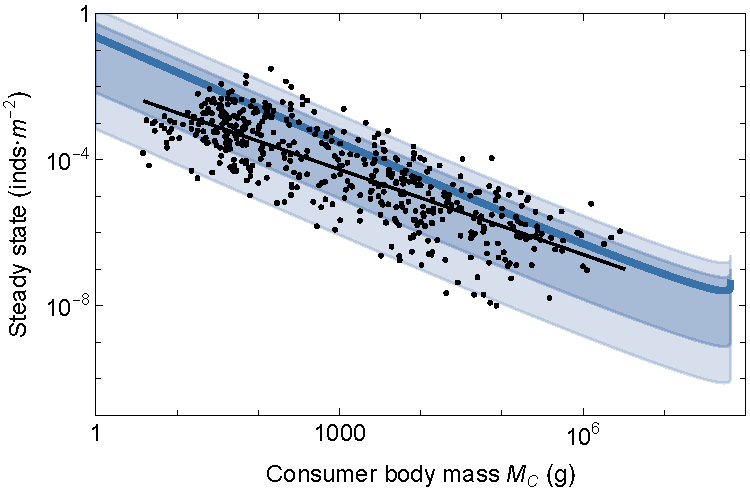
\includegraphics[width=0.5\textwidth]{fig_consumer2d_resources.pdf}
\caption{Model predictions of mammalian steady states compared to observational data from Damuth (REF).}
\label{fig:2ddensities}
\end{figure}


\begin{figure}[h!]
    % \centering
    % 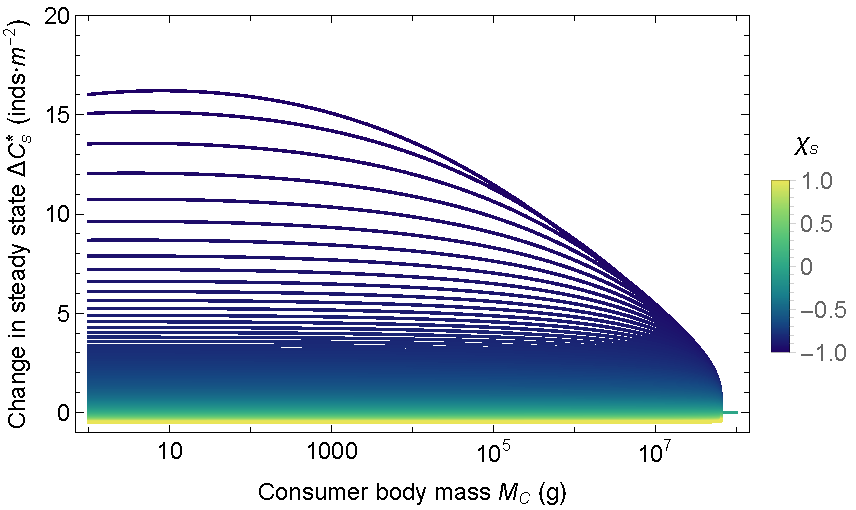
\includegraphics[width=0.5\textwidth]{fig_starverelative.pdf}
    \caption{Caption}
    \label{fig:starve}
\end{figure}


\begin{figure}[h!]
    % \centering
    % 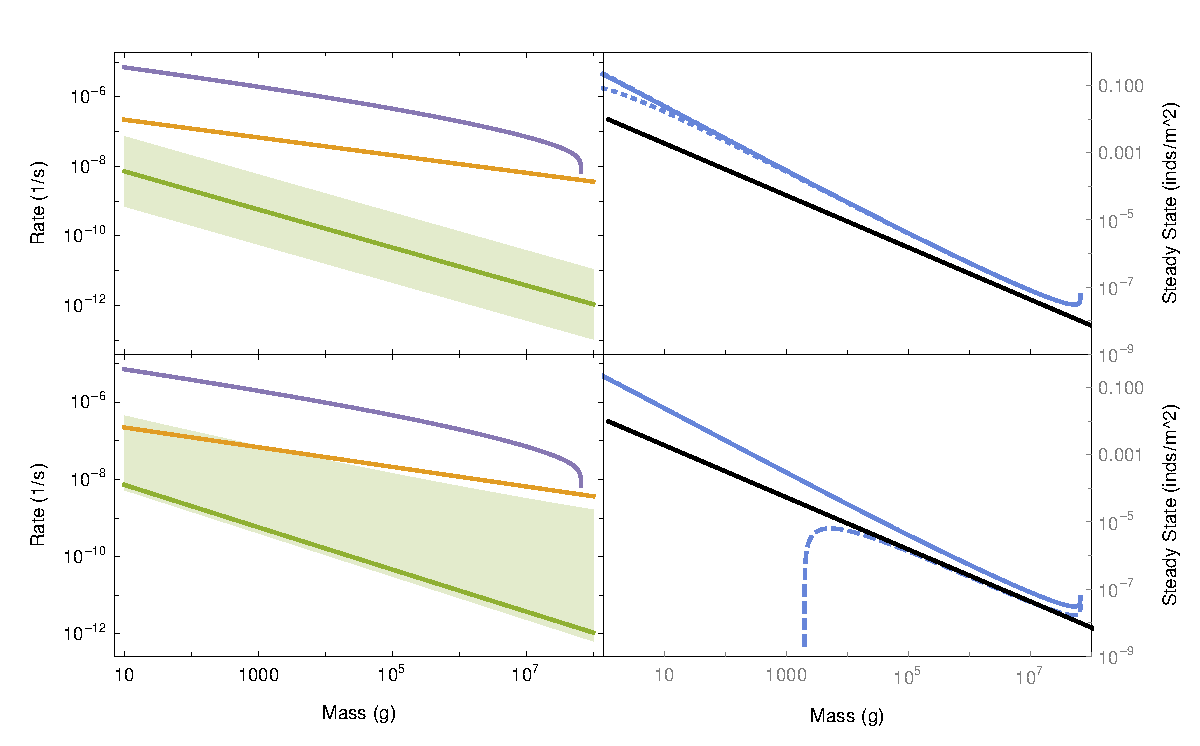
\includegraphics[width=0.9\textwidth]{joined_survivorship.pdf}
    \caption{Caption}
    \label{fig:naturalmort}
\end{figure}


\begin{figure}[h!]
%   \centering
%   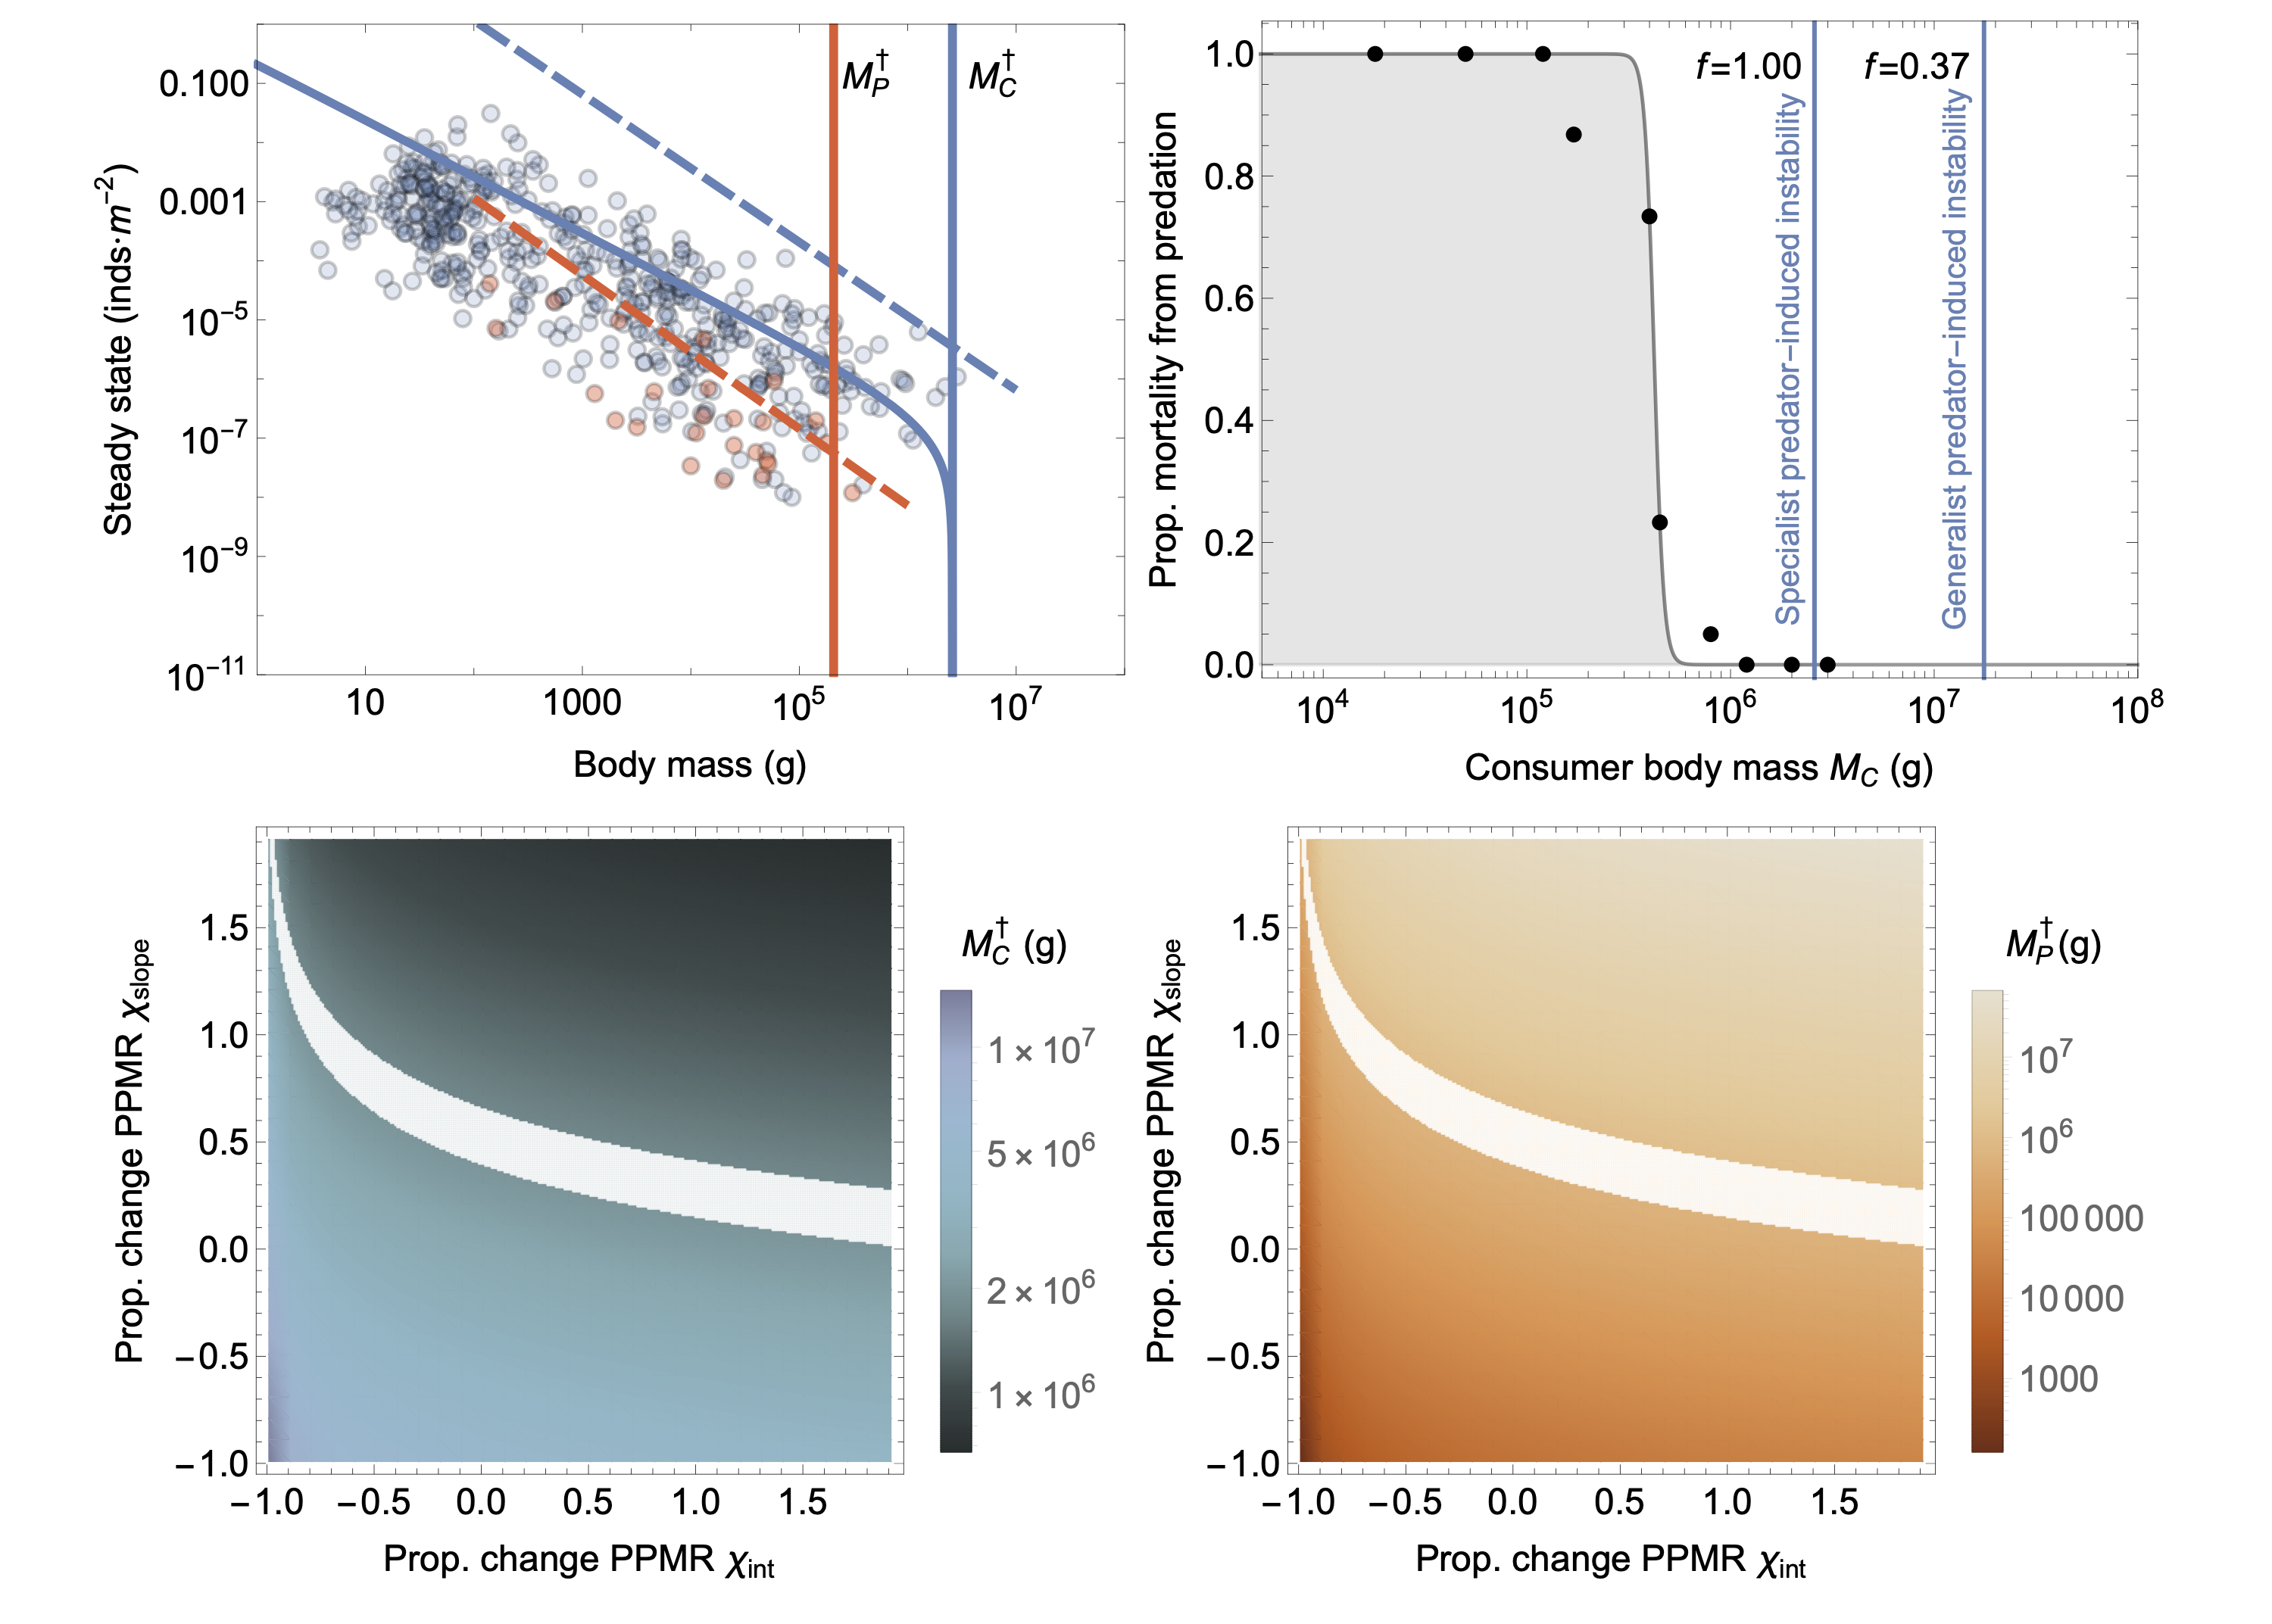
\includegraphics[width=1\textwidth]{fig_predation_alltogether.png}
  \caption{
	  A) Empirical mammalian herbivore (blue points) and predator (red points) mass-densities shown alongside the theoretical maximum herbivore $C^{\rm max}$ and predator $P^{\rm max}$ densities as a function of body size. 
	  The solid blue curve denotes the predicted herbivore consumer steady state $C^*(M_C)$, assuming mortality from starvation, life-history effects, and predation.
	  Predicted herbivore $M_C^\dagger$ and predator $M_P^\dagger$ size thresholds (blue and red vertical lines, respectively) reveal where the herbivore consumer population is no longer able to support a predator population. 
	  The blue shaded region denotes `mega' size classes $>1\times10^5$ g.
	  B) Percent mortality from predation for Serengeti herbivores (redrawn from Sinclair et al. \citep{Sinclair2003}) as a function of body mass $M_C$. Gray shaded region denotes a sigmoidal fit to the data with the inflection at $4.22\times10^5$ g. Vertical lines show herbivore size threshold under the assumption of predator specialization ($f=1.00$, where $M_C^\dagger=2.58\times10^6$) and an example of generalization ($f=0.37$, where $M_C^\dagger=1.75\times10^7$).
	  C) Threshold herbivore sizes $M_C^\dagger$ across a range of PPMR relationships, where ${\rm E}(M_P|M_C) = p_0(1+\chi_{\rm int}) M_C^{p_1(1+\chi_{\rm slope})}$.
	  White shaded region denotes megatrophic threshold sizes, where both $M_C^\dagger,M_P^\dagger > 6\times10^5$ g. 
	  D) As in C), but showing the corresponding threshold carnivore sizes $M_P^\dagger$.
  }
  \label{fig:predrate}
\end{figure}


\begin{figure}[h!]
    % \centering
    % 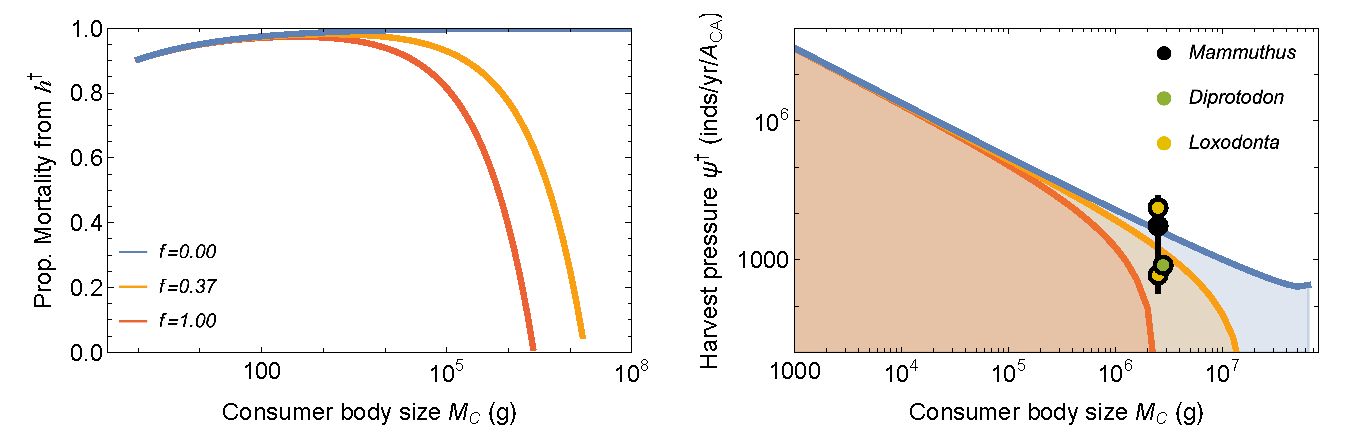
\includegraphics[width=1\textwidth]{fig_harvest.pdf}
    \caption{Caption}
    \label{fig:harvest}
\end{figure}





% \begin{figure}[h!]
% %\includegraphics{horn-of-okapi}
% \caption{Figure legends can be longer than the titles of tables. However, they should not be excessively long.}
% \label{Fig:OkapiHorn}
% \end{figure}


%%%%%%%%%%%%%%%%%%%%%
% Videos
%%%%%%%%%%%%%%%%%%%%%
% If you have videos, journal style for them is similar to that for
% figures. You'll want to include a still image (such as a JPEG)
% to give your readers a preview of what the video looks like.

%%%%% Include the text below if you have videos

% \renewcommand{\figurename}{Video} 
% \setcounter{figure}{0}
% % Thanks to Flo Debarre for the pro tip of putting
% % \renewcommand{\figurename}{Video} before the Video legend and
% % \renewcommand{\figurename}{Figure} after it!

% \begin{figure}[h!]
% %\includegraphics{VideoScreengrab.jpg}
% \caption{Video legends can follow the same principles as figure legends. Counters should be set and reset so that videos and figures are enumerated separately.}
% \label{VideoExample}
% \end{figure}

\renewcommand{\figurename}{Figure}
\setcounter{figure}{1}

%%%%% Include the above if you have videos











% \begin{figure}[h!]
% %\includegraphics{elegance}
% \caption{In this way, figure legends can be listed at the end of the document, with references that work, even though the graphic itself should be included for final files after acceptance. Instead, upload the relevant figure files separately to Editorial Manager; Editorial Manager should insert them at the end of the PDF automatically.}
% \label{Fig:AnotherFigure}
% \end{figure}

\subsection*{Online figure legends}

\renewcommand{\thefigure}{A\arabic{figure}}
\setcounter{figure}{0}

% \begin{figure}[h!]
% %\includegraphics{jumps20m}
% \caption{\textit{A}, the quick red fox proceeding to jump 20~m straight into the air over not one, but several lazy dogs. \textit{B}, the quick red fox landing gracefully despite the skepticism of naysayers.}
% \label{Fig:Jumps}
% \end{figure}

% \begin{figure}[h!]
% %\includegraphics{jumps20m}
% \caption{The quicker the red fox jumps, the likelier it is to land near an okapi. For further details, see \citept{LemKapEx07}.}
% \label{Fig:JumpsOk}
% \end{figure}


\begin{figure}[h!]
% \begin{subfigure}
% 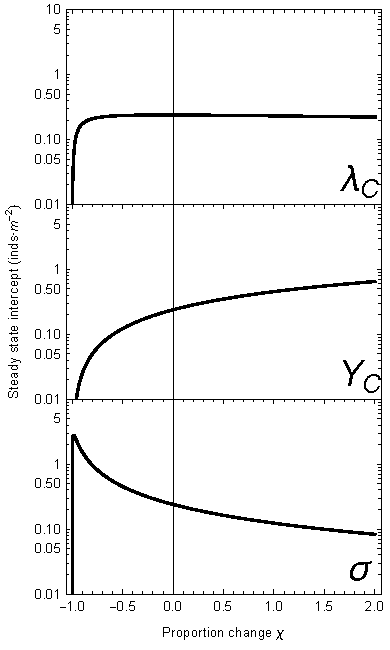
\includegraphics[width=0.45\textwidth]{fig_intmod.pdf}
% \end{subfigure}
% \begin{subfigure}
% 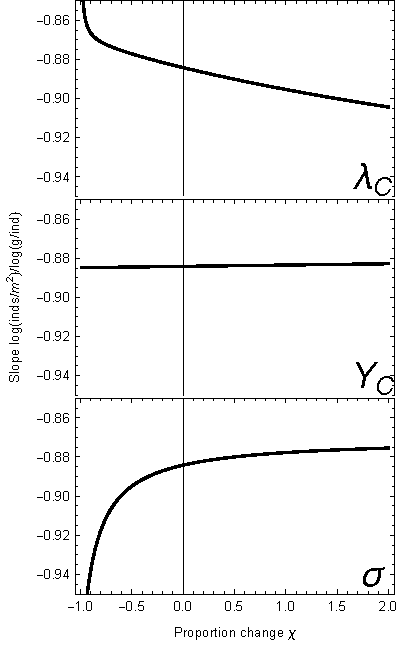
\includegraphics[width=0.45\textwidth]{fig_slopemod.pdf}
% % \includegraphics[width=0.9\textwidth]{starvation_reproductionrates.png}
% \end{subfigure}
\caption{The effects of changes to metabolic parameters on the prediction of the mass-density relationship.}
\label{fig:corr}
\end{figure}



\begin{figure}[h!]
%   \centering
%   \includegraphics[width=0.6\textwidth]{fig_meanpredsize34_log.pdf}
  \caption{
	 Expected predator masses for contemporary large-bodied ($>10^5$ g) terrestrial predators and prey. 
	 Expected predator sizes as a function of herbivore size class were determined by reconstructing dietary samples from observed trophic interactions for cheetah, wild dogs, dholes, leopards, hyenas, lions, and tigers from \citep{Hayward2008} (REF others), where masses for both predators and prey were allowed to vary $\pm 20\%$ from measured estimates.
	 The blue line denotes the best fit relationship, given by ${\rm E}(M_P|M_C) = p_0 M_C^{p_1}$, where $p_0 = 11786.8$ g and $p_1 = 0.194$.
	 The red line represents a modified PPMR where $p_0^\prime = p_0(1+\chi_{\rm int})$ and $p_1^\prime = p_1(1+\chi_{\rm slope})$ where $\chi_{\rm int} = 0.97$ and $\chi_{\rm slope} = 1.50$ that allows megatrophic interactions and resides within the white band displayed in Fig. \ref{fig:predrate}C,D.
	 This relationship is entirely hypothetical, but does not stray far from observations of contemporary species, describes megapredators that predate on megaherbivores, and results in threshold herbivore and carnivore size classes that permit dynamically feasible megatrophic interactions.
	 The black line denotes the 1:1 line.
  }
  \label{fig:ppmr}
\end{figure}

\begin{figure}[h!]
%   \centering
%   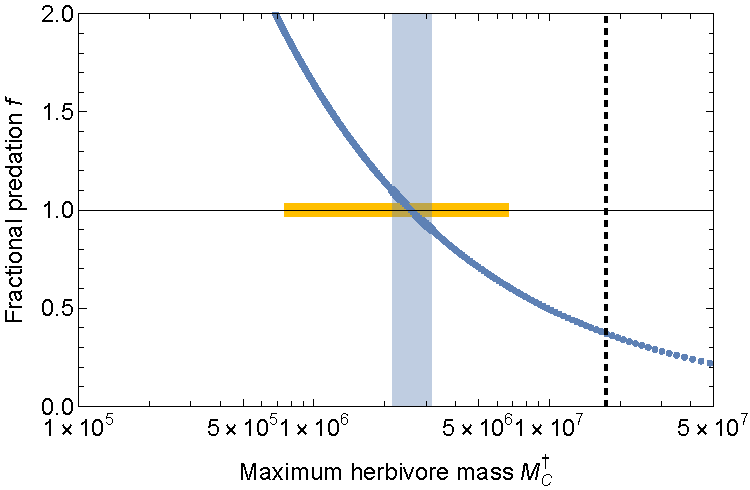
\includegraphics[width=0.6\textwidth]{fig_maxpreyvar.pdf}
  \caption{
	  The effect of changing the reliance of predator growth $f$ on the single herbivore consumer population. If $f=1$, the predator solely relies on the herbivore consumer. If $0<f<1$, the predator relies on the herbivore population to support a fraction of its growth. If $f>1$, the predator is removing more biomass than is necessary to support its growth.
	  Blue region denotes herbivore threshold mass range characterizing $f=1 \pm 0.1$.
	  Yellow line denotes the mass range of contemporary elephants.
	  Vertical dashed line denotes the size of the largest terrestrial mammal (Deinotherium at ca. $1.74\times 10^7$, corresponding to $f=0.37$, such that a predator is supporting a little more than 1/3 of its growth from the herbivore consumer.
  }
  \label{fig:maxpreyvar}
\end{figure}

\begin{figure}[h!]
%   \centering
%   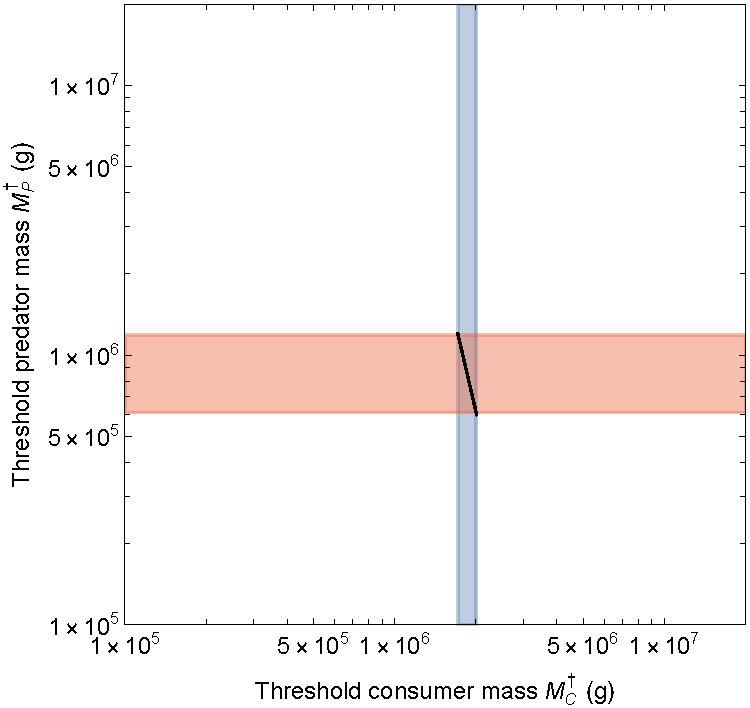
\includegraphics[width=0.6\textwidth]{fig_megamammal.pdf}
  \caption{
    Mass ranges corresponding to feasible megatrophic interactions (where herbivore and predator threshold masses are $> 6\times10^5$ g) across variations to the assumed predator-prey mass ratio (PPMR), demarcated by the white bands in Fig. \ref{fig:predrate}C,D, and under the assumption specialist predation ($f=1$). 
% 	  The range of herbivore and carnivore threshold size classes where both species are characterized by mega- body mass ($>6\times10^5$ g) under the condition of predator specialization and across variable PPMRs, where ${\rm E}(M_P|M_C) = p_0(1+\chi_{\rm int}) M_C^{p_1(1+\chi_{\rm slope})}$ and both $\chi_{\rm int}$ and $\chi_{\rm slope} \in (-0.99,2)$.
  }
  \label{fig:megamammal}
\end{figure}

\begin{figure}[h!]
%   \centering
%   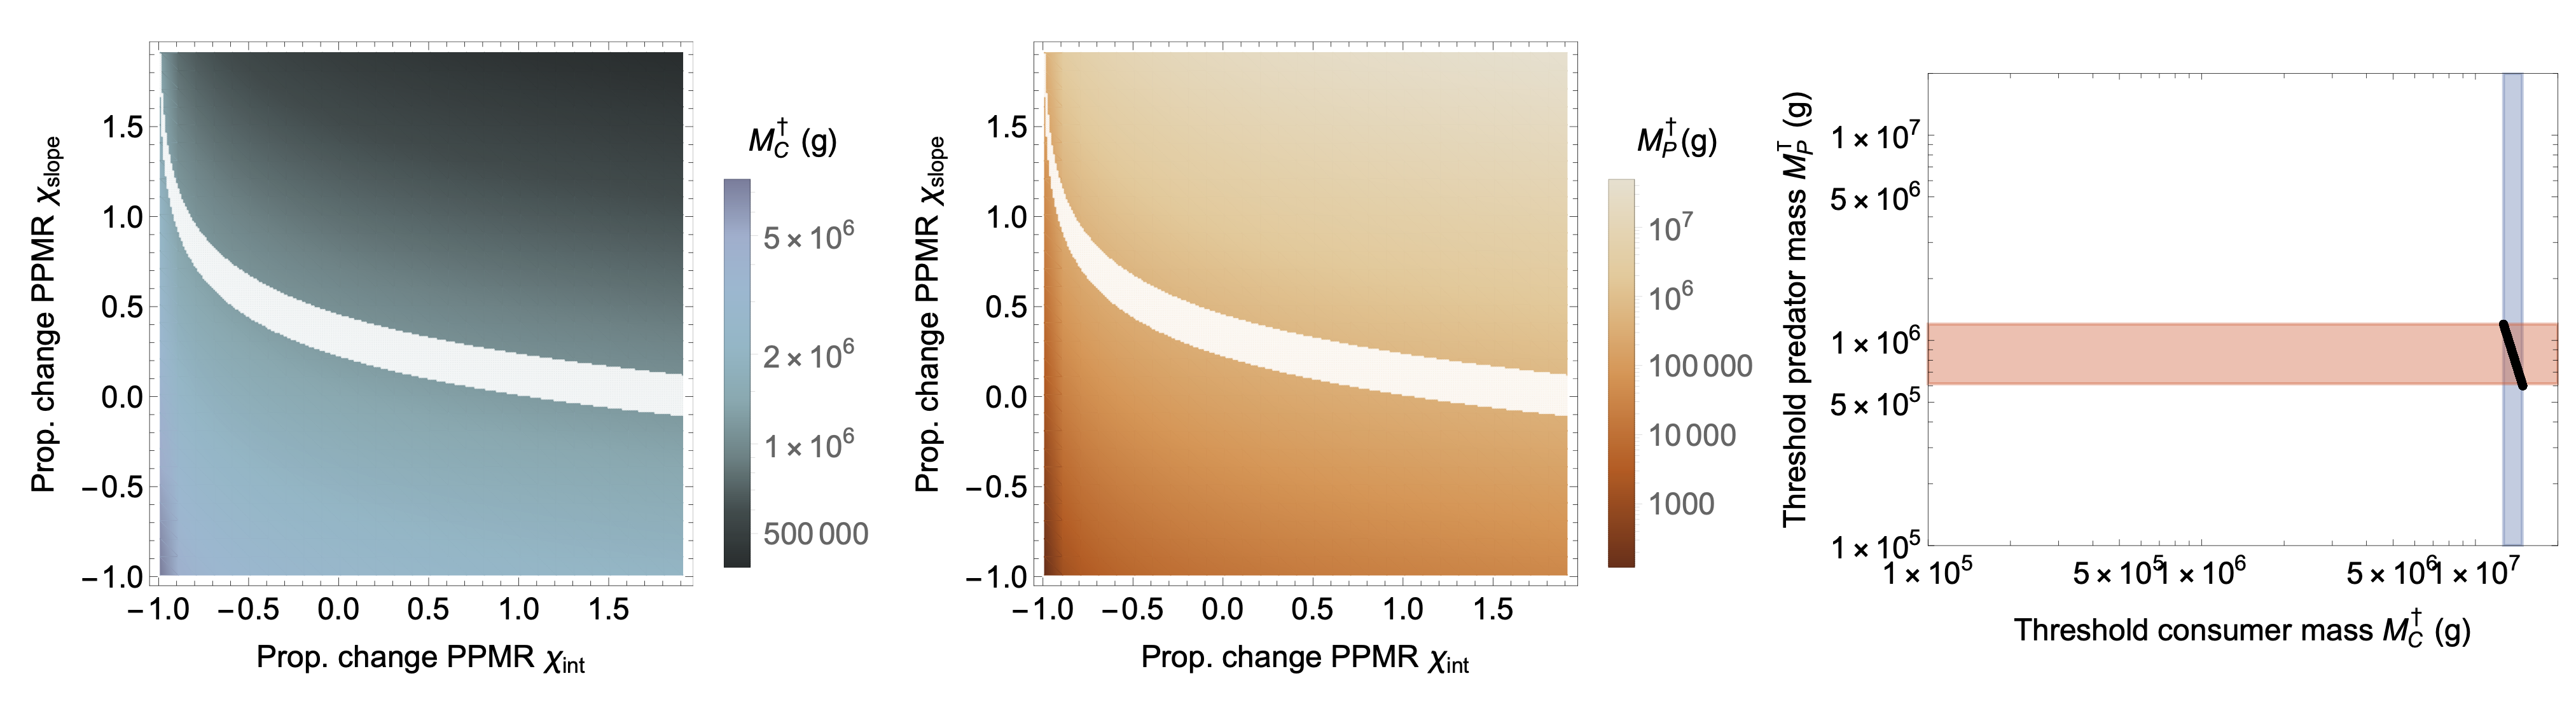
\includegraphics[width=1\textwidth]{fig_megamammal_generalist.pdf}
  \caption{
    The effects of predator generalization on A) threshold herbivore mass $M_C^\dagger$ and B) threshold predator mass $M_P^\dagger$ across variable PPMRs, where ${\rm E}(M_P|M_C) = p_0(1+\chi_{\rm int}) M_C^{p_1(1+\chi_{\rm slope})}$ and both $\chi_{\rm int}$ and $\chi_{\rm slope} \in (-0.99,2)$.
    White bands denote regions of $\chi_{\rm int}$ and $\chi_{\rm slope}$ where megatrophic interactions are feasible (both perdator and herbivore threshold masses are $> 6\times10^5$ g).
    C) Mass ranges corresponding to feasible megatrophic interactions in the white bands in A and B.
  }
  \label{fig:megamammalgen}
\end{figure}

\begin{figure}[h!]
%   \centering
% 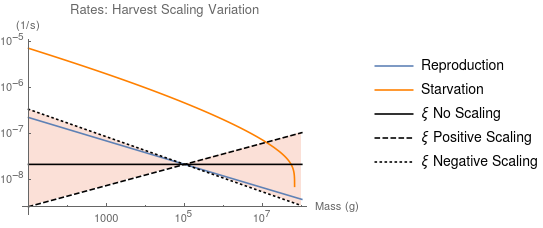
\includegraphics[width=0.9\textwidth]{harvest_scaling_plot.png}
\caption{
  }
  \label{fig:harvestscaling}
\end{figure}



\renewcommand{\thefigure}{B\arabic{figure}}
\setcounter{figure}{0}

\end{document}
